\documentclass[]{jarticle}          % 一段組
%\documentclass[twocolumn]{jarticle} % 二段組

\textwidth 180mm
\textheight 255mm
\oddsidemargin -12mm
\topmargin -15mm
\columnsep 10mm

%\vspace{0.5cm} % 一段組の場合はコメントアウトした方が体裁がよいx
%] % 一段組の場合はコメントアウトする

\usepackage{styles/labheadings}
\usepackage[dvipdfmx]{graphicx,color}
\usepackage{amsmath,amssymb}
\usepackage{url}
% 追加
\usepackage[hang,small,bf]{caption}
\usepackage[subrefformat=parens]{subcaption}
\usepackage{float}
\captionsetup{compatibility=false}

\newcommand{\aU}{\mbox{\boldmath $a$}}
\newcommand{\bU}{\mbox{\boldmath $b$}}
\newcommand{\cU}{\mbox{\boldmath $c$}}
\newcommand{\dU}{\mbox{\boldmath $d$}}
\newcommand{\eU}{\mbox{\boldmath $e$}}
\newcommand{\fU}{\mbox{\boldmath $f$}}
\newcommand{\gU}{\mbox{\boldmath $g$}}
\newcommand{\hU}{\mbox{\boldmath $h$}}
\newcommand{\iU}{\mbox{\boldmath $i$}}
\newcommand{\jU}{\mbox{\boldmath $j$}}
\newcommand{\kU}{\mbox{\boldmath $k$}}
\newcommand{\lU}{\mbox{\boldmath $l$}}
\newcommand{\mU}{\mbox{\boldmath $m$}}
\newcommand{\nU}{\mbox{\boldmath $n$}}
\newcommand{\oU}{\mbox{\boldmath $o$}}
\newcommand{\pU}{\mbox{\boldmath $p$}}
\newcommand{\qU}{\mbox{\boldmath $q$}}
\newcommand{\rU}{\mbox{\boldmath $r$}}
\newcommand{\sU}{\mbox{\boldmath $s$}}
\newcommand{\tU}{\mbox{\boldmath $t$}}
\newcommand{\uU}{\mbox{\boldmath $u$}}
\newcommand{\vU}{\mbox{\boldmath $v$}}
\newcommand{\wU}{\mbox{\boldmath $w$}}
\newcommand{\xU}{\mbox{\boldmath $x$}}
\newcommand{\yU}{\mbox{\boldmath $y$}}
\newcommand{\zU}{\mbox{\boldmath $z$}}
\newcommand{\AU}{\mbox{\boldmath $A$}}
\newcommand{\BU}{\mbox{\boldmath $B$}}
\newcommand{\CU}{\mbox{\boldmath $C$}}
\newcommand{\DU}{\mbox{\boldmath $D$}}
\newcommand{\EU}{\mbox{\boldmath $E$}}
\newcommand{\FU}{\mbox{\boldmath $F$}}
\newcommand{\GU}{\mbox{\boldmath $G$}}
\newcommand{\HU}{\mbox{\boldmath $H$}}
\newcommand{\IU}{\mbox{\boldmath $I$}}
\newcommand{\JU}{\mbox{\boldmath $J$}}
\newcommand{\KU}{\mbox{\boldmath $K$}}
\newcommand{\LU}{\mbox{\boldmath $L$}}
\newcommand{\MU}{\mbox{\boldmath $M$}}
\newcommand{\NU}{\mbox{\boldmath $N$}}
\newcommand{\OU}{\mbox{\boldmath $O$}}
\newcommand{\PU}{\mbox{\boldmath $P$}}
\newcommand{\QU}{\mbox{\boldmath $Q$}}
\newcommand{\RU}{\mbox{\boldmath $R$}}
\newcommand{\SU}{\mbox{\boldmath $S$}}
\newcommand{\TU}{\mbox{\boldmath $T$}}
\newcommand{\UU}{\mbox{\boldmath $U$}}
\newcommand{\VU}{\mbox{\boldmath $V$}}
\newcommand{\WU}{\mbox{\boldmath $W$}}
\newcommand{\XU}{\mbox{\boldmath $X$}}
\newcommand{\YU}{\mbox{\boldmath $Y$}}
\newcommand{\ZU}{\mbox{\boldmath $Z$}}
\newcommand{\epU}{\mbox{\boldmath $\epsilon$}}
\newcommand{\taU}{\mbox{\boldmath $\tau$}}
\newcommand{\etU}{\mbox{\boldmath $\eta$}}
\newcommand{\xiU}{\mbox{\boldmath $\xi$}}
\newcommand{\wwU}{\mbox{\boldmath $\omega$}}
\newcommand{\WwU}{\mbox{\boldmath $\Omega$}}
\newcommand{\lmU}{\mbox{\boldmath $\lambda$}}
\newcommand{\LmU}{\mbox{\boldmath $\Lambda$}}
\newcommand{\PiU}{\mbox{\boldmath $\Pi$}}
\newcommand{\SgU}{\mbox{\boldmath $\Sigma$}}
\newcommand{\thU}{\mbox{\boldmath $\theta$}}
\newcommand{\ThU}{\mbox{\boldmath $\Theta$}}
\newcommand{\roU}{\mbox{\boldmath $\rho$}}
\newcommand{\nuU}{\mbox{\boldmath $\nu$}}
\newcommand{\ones}{{\bf 1}}
\newcommand{\zr}{{\bf 0}}
\newcommand{\eq}{\begin{equation}}
\newcommand{\en}{\end{equation}}
\newcommand{\eqa}{\begin{eqnarray}}
\newcommand{\ena}{\end{eqnarray}}
\newcommand{\xx}{\makebox[1cm]{}}
\newcommand{\xm}{\makebox[0.5cm]{}}
\newcommand{\x}{\makebox[0.2cm]{}}
\newcommand{\tr}{{\rm tr}}
\newcommand{\sgn}{{\rm sgn}}
\newcommand{\ad}{{\rm ad}}
\newcommand{\rank}{{\rm rank}}
\newcommand{\diag}{{\rm diag}}
\newcommand{\lbr}{\left(\begin{array}}
\newcommand{\rbr}{\end{array}\right)}
\newcommand{\Proof}{\noindent{\em Proof\/}}
\newcommand{\Solution}{\noindent{\em Solution}}
\newcommand{\Derivation}{\noindent{\em Derivation}}
\newcommand{\msp}{\vspace*{\medskipamount}\\}
\newcommand{\qed}{\hspace*{\fill}$\Box$}
\newcommand{\aX}{{\bf a}}
\newcommand{\bX}{{\bf b}}
\newcommand{\cX}{{\bf c}}
\newcommand{\dX}{{\bf d}}
\newcommand{\eX}{{\bf e}}
\newcommand{\fX}{{\bf f}}
\newcommand{\gX}{{\bf g}}
\newcommand{\hX}{{\bf h}}
\newcommand{\iX}{{\bf i}}
\newcommand{\jX}{{\bf j}}
\newcommand{\kX}{{\bf k}}
\newcommand{\lX}{{\bf l}}
\newcommand{\mX}{{\bf m}}
\newcommand{\nX}{{\bf n}}
\newcommand{\oX}{{\bf o}}
\newcommand{\pX}{{\bf p}}
\newcommand{\qX}{{\bf q}}
\newcommand{\rX}{{\bf r}}
\newcommand{\sX}{{\bf s}}
\newcommand{\tX}{{\bf t}}
\newcommand{\uX}{{\bf u}}
\newcommand{\vX}{{\bf v}}
\newcommand{\wX}{{\bf w}}
\newcommand{\xX}{{\bf x}}
\newcommand{\yX}{{\bf y}}
\newcommand{\zX}{{\bf z}}
\newcommand{\AX}{{\bf A}}
\newcommand{\BX}{{\bf B}}
\newcommand{\CX}{{\bf C}}
\newcommand{\DX}{{\bf D}}
\newcommand{\EX}{{\bf E}}
\newcommand{\FX}{{\bf F}}
\newcommand{\GX}{{\bf G}}
\newcommand{\HX}{{\bf H}}
\newcommand{\IX}{{\bf I}}
\newcommand{\JX}{{\bf J}}
\newcommand{\KX}{{\bf K}}
\newcommand{\LX}{{\bf L}}
\newcommand{\MX}{{\bf M}}
\newcommand{\NX}{{\bf N}}
\newcommand{\OX}{{\bf O}}
\newcommand{\PX}{{\bf P}}
\newcommand{\QX}{{\bf Q}}
\newcommand{\RX}{{\bf R}}
\newcommand{\SX}{{\bf S}}
\newcommand{\TX}{{\bf T}}
\newcommand{\UX}{{\bf U}}
\newcommand{\VX}{{\bf V}}
\newcommand{\WX}{{\bf W}}
\newcommand{\XX}{{\bf X}}
\newcommand{\YX}{{\bf Y}}
\newcommand{\ZX}{{\bf Z}}

% report.texと同じディレクトリにnumerical_definition.texを入れておけば上の書き方でもいいはずです

\usepackage[
  dvipdfm,
  bookmarks=true,
  bookmarksnumbered=true,
  colorlinks=true]{hyperref}
\AtBeginDvi{\special{pdf:tounicode EUC-UCS2}}

\pagestyle{labheadings}
\headerleft{2次元フロアマップからのシーンの3次元モデルの作成}   % ヘッダの左側のタイトル
\headerright{2024年12月11日}  % ヘッダの右側のタイトル

\begin{document}

%\twocolumn % 一段組の場合はコメントアウトする

\vspace*{2ex}
\begin{center}
 {\Large \bf 3次元モデルの改良}\\ % タイトル
 \vspace*{5mm}
 {\large M1 田川幸汰}% 発表者名
\end{center}

%\vspace{0.5cm} % 一段組の場合はコメントアウトした方が体裁がよいx
%] % 一段組の場合はコメントアウトする

%新しく作成したコマンド
% \newcommand{\reffig}[1]{\hyperref[#1]{図\ref{#1}}}
% \newcommand{\refeq}[1]{\hyperref[#1]{式(\ref{#1})}}
% \newcommand{\reftab}[1]{\hyperref[#1]{表\ref{#1}}}
% \newcommand{\refsec}[1]{\hyperref[#1]{\ref{#1}章}}
% \newcommand{\refsubsec}[1]{\hyperref[#1]{\ref{#1}節}}

% 数式
%\begin{equation}
%  数式記述  
%  \label{ラベル名}
%\end{equation}

% 図
% \begin{figure}[!ht]
%   \begin{center}
%     \includegraphics[scale=0.5]{figures/画像ファイル名}
%     \caption{キャプション名}
%     \label{ラベル名}
%   \end{center}
% \end{figure}

% リスト
% \begin{enumerate or itemize}
%   \item 
% \end{enumerate or itemize}
\section{概要}
前回の進捗報告において作成したテクスチャを\hyperref[one]{図\ref{one}}に示す。
また、これらのテクスチャを用いて生成した3次元モデルを\hyperref[two]{図\ref{two}}に示す。
各全方位カメラで取得したテクスチャは、個別に見るとおおむね正しい位置に適切に配置されていることが確認された。
しかし、これらを組み合わせて3次元モデルとして統合した場合、いくつかの課題が顕在化した。
まず、全方位カメラ間で取得されたテクスチャに明るさの違いが見られ、モデル全体で輝度が統一されていないことが確認された。
また、異なるカメラによるテクスチャの境界において、位置のずれが顕著に現れており、モデル全体の一体感を損ねる結果となった。
\begin{figure}[H]
  \begin{center}
    \begin{tabular}{cc}
      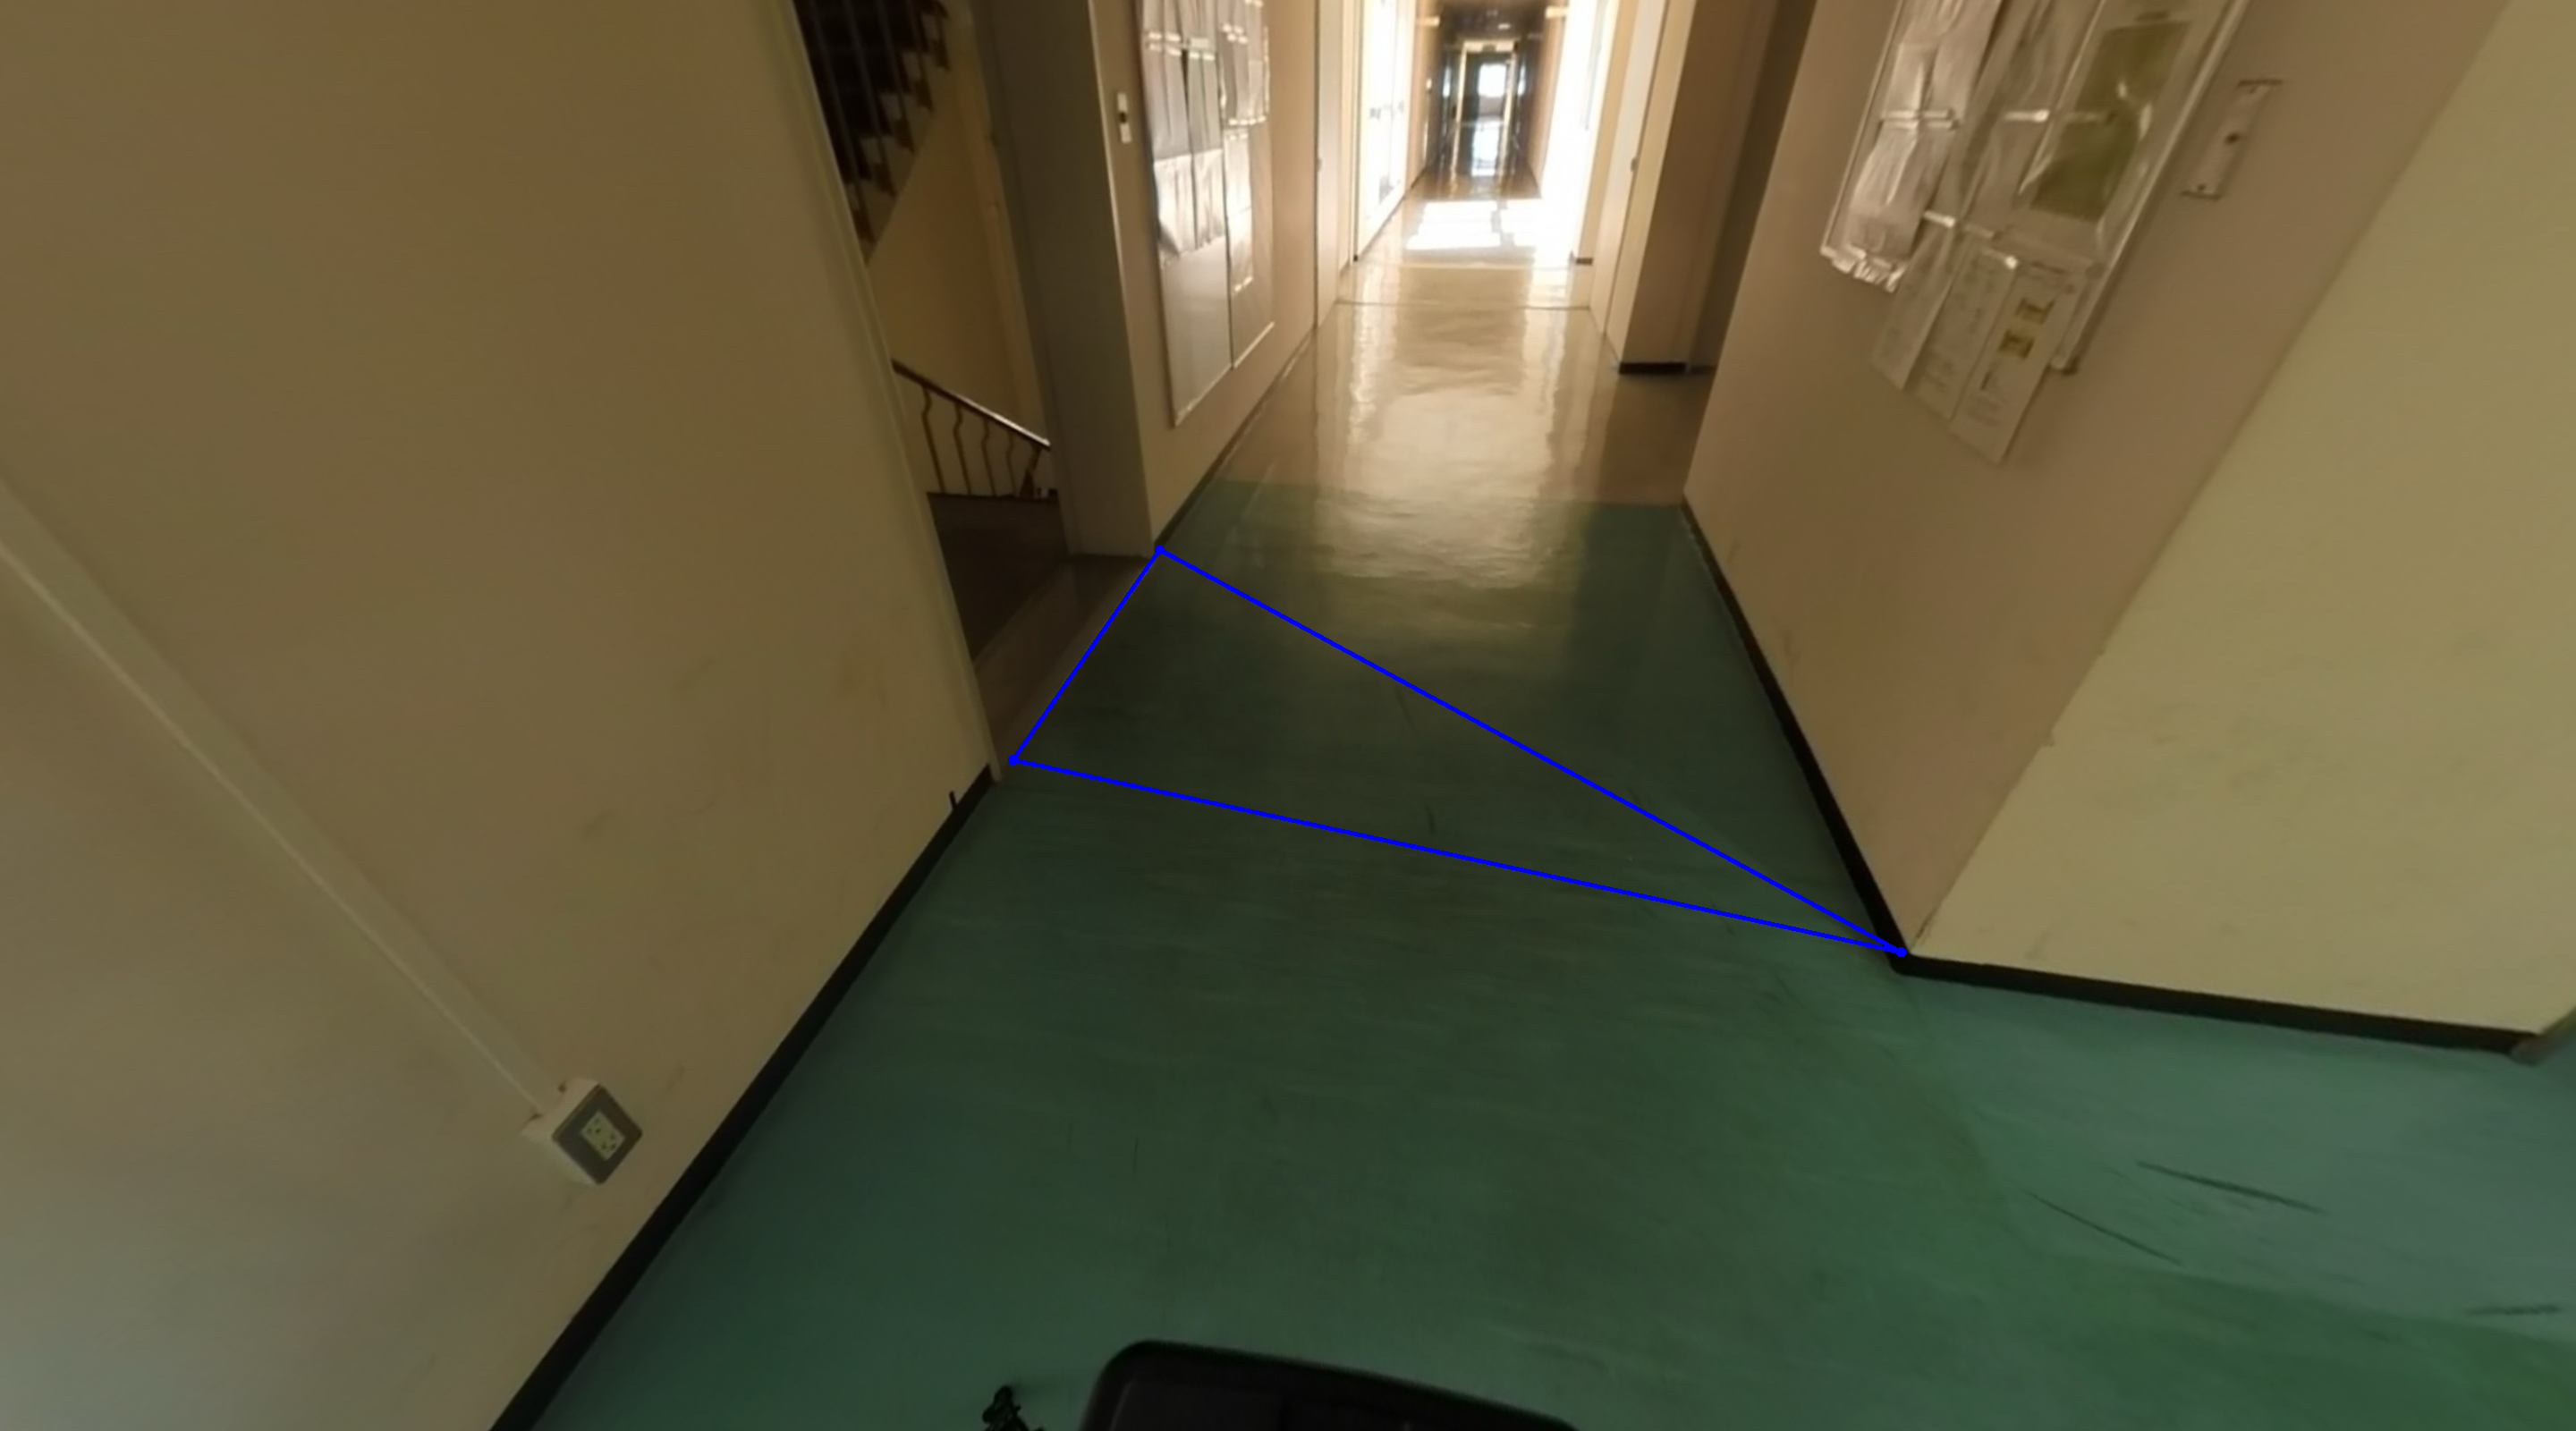
\includegraphics[width=0.3\textwidth]{figures/texture_0_0.png}&
      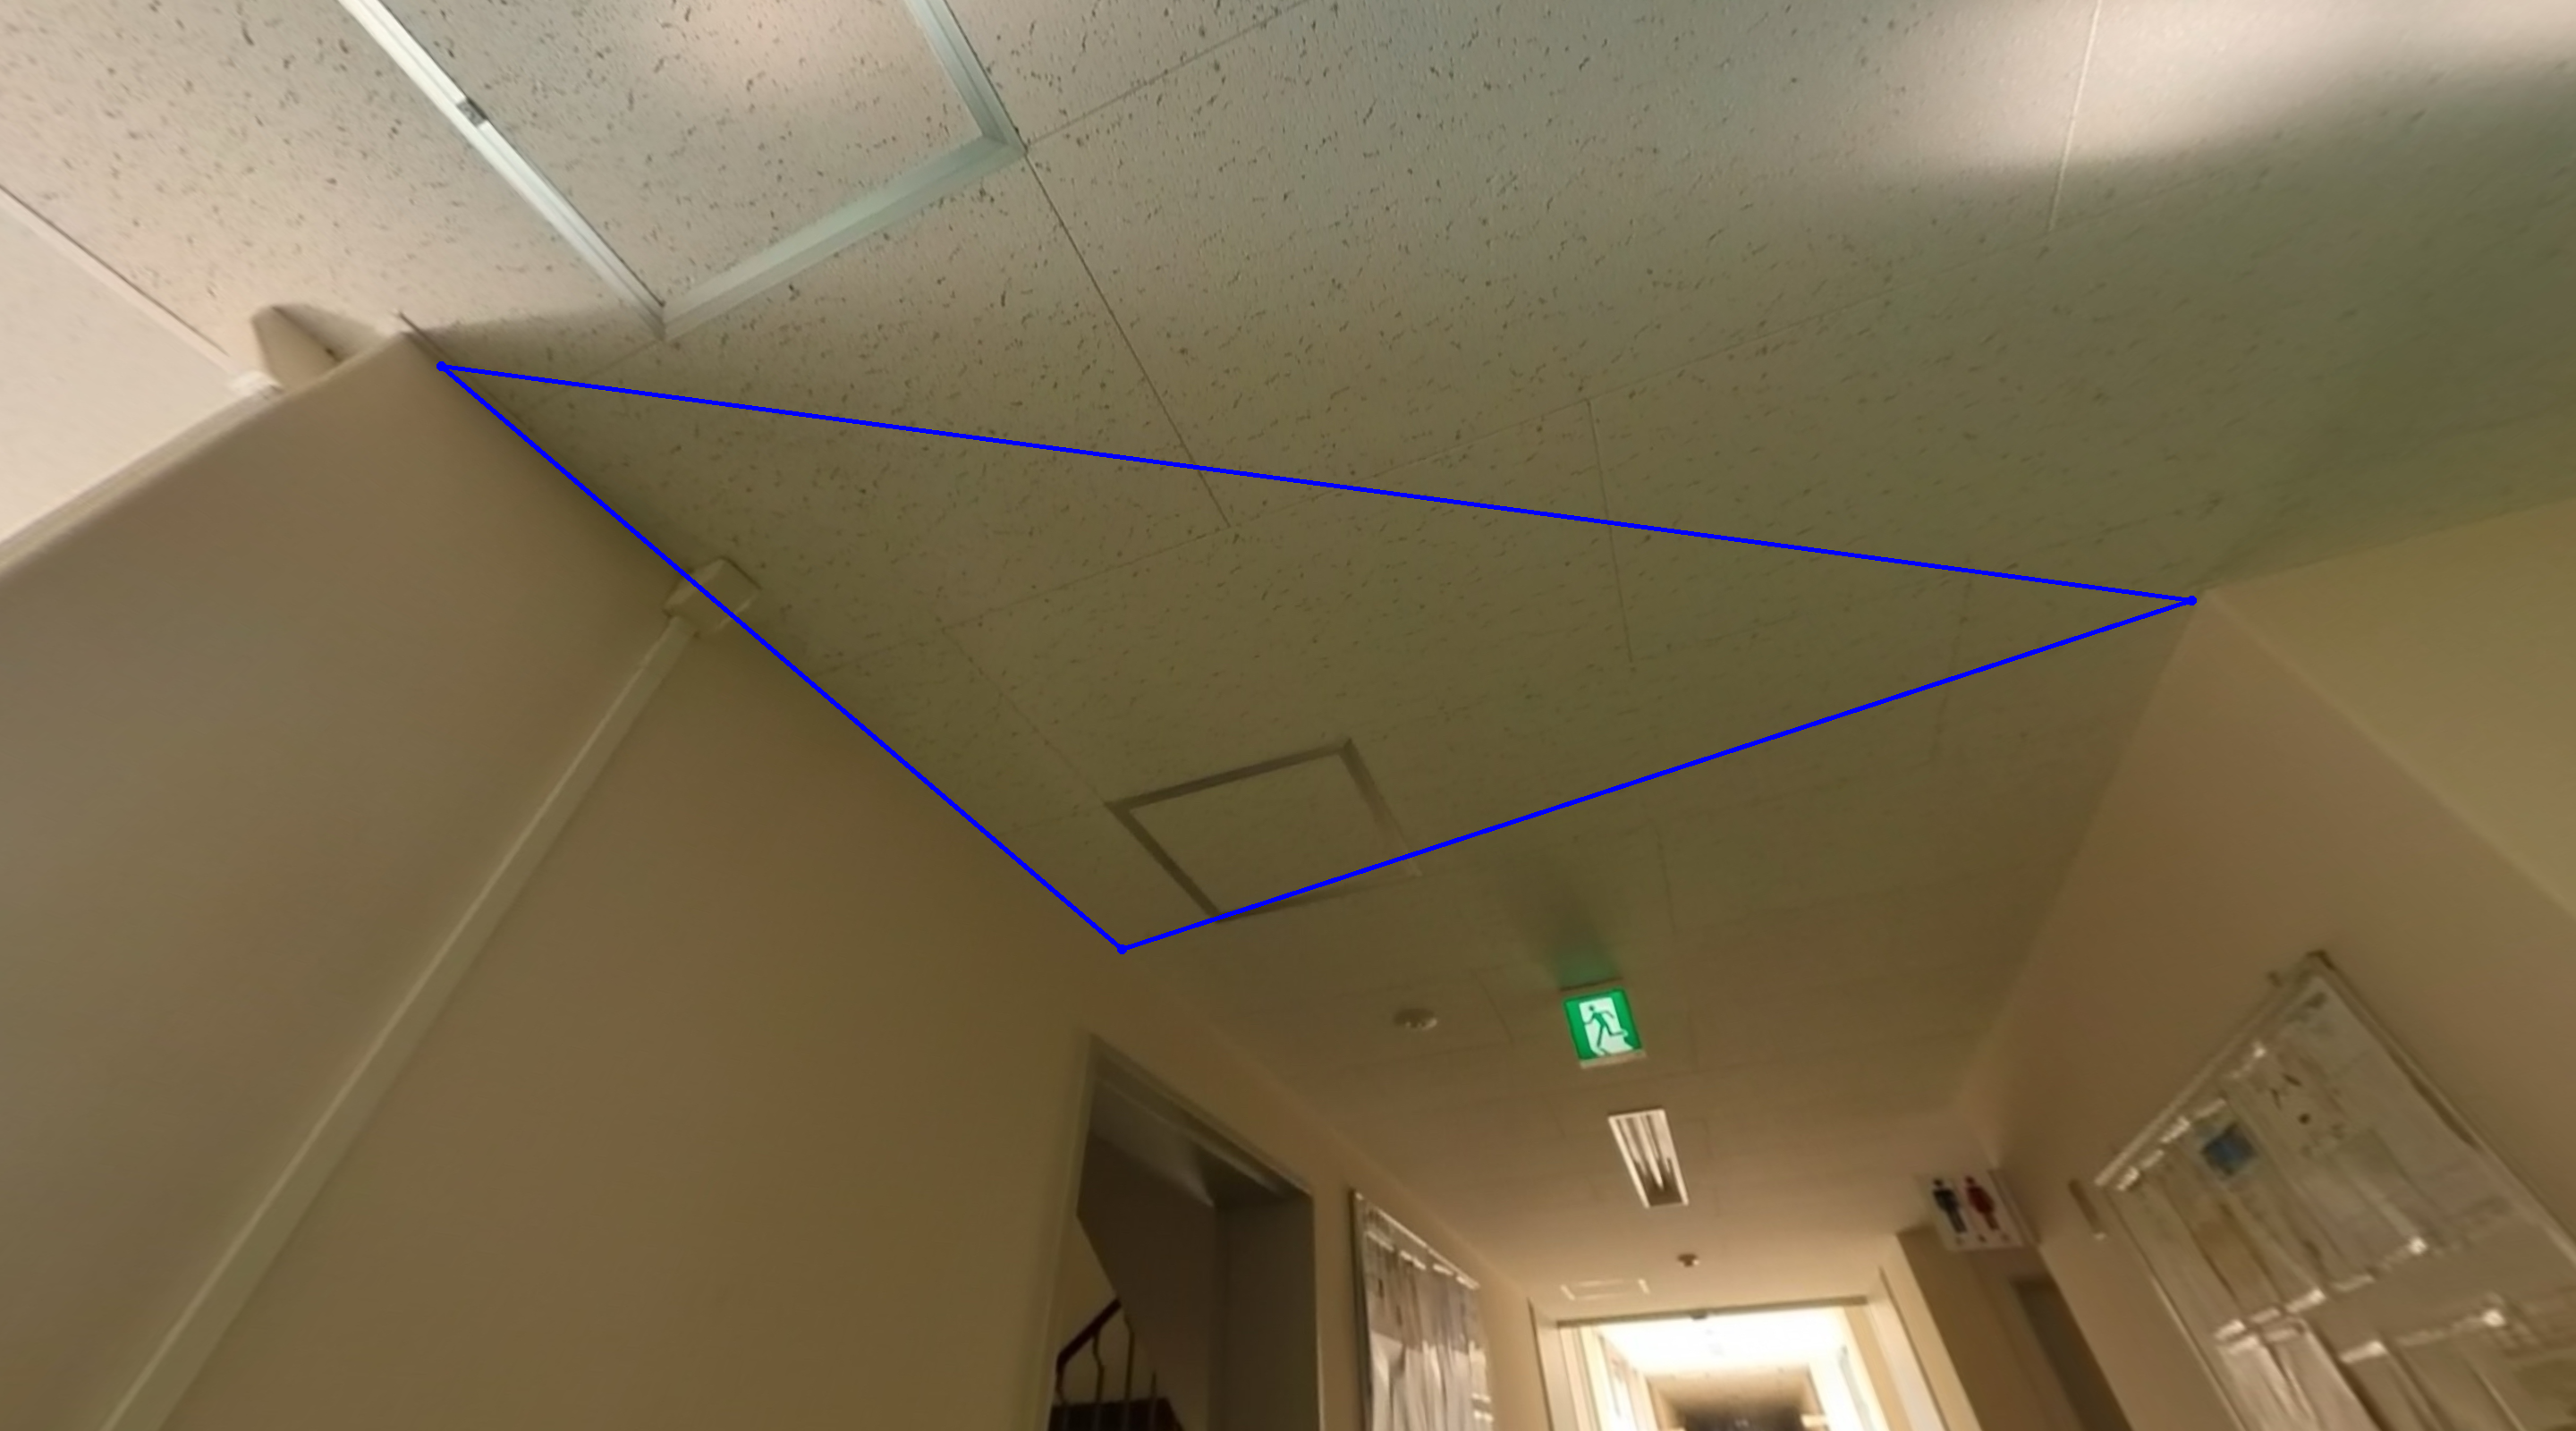
\includegraphics[width=0.3\textwidth]{figures/texture_0_5.png}\\
      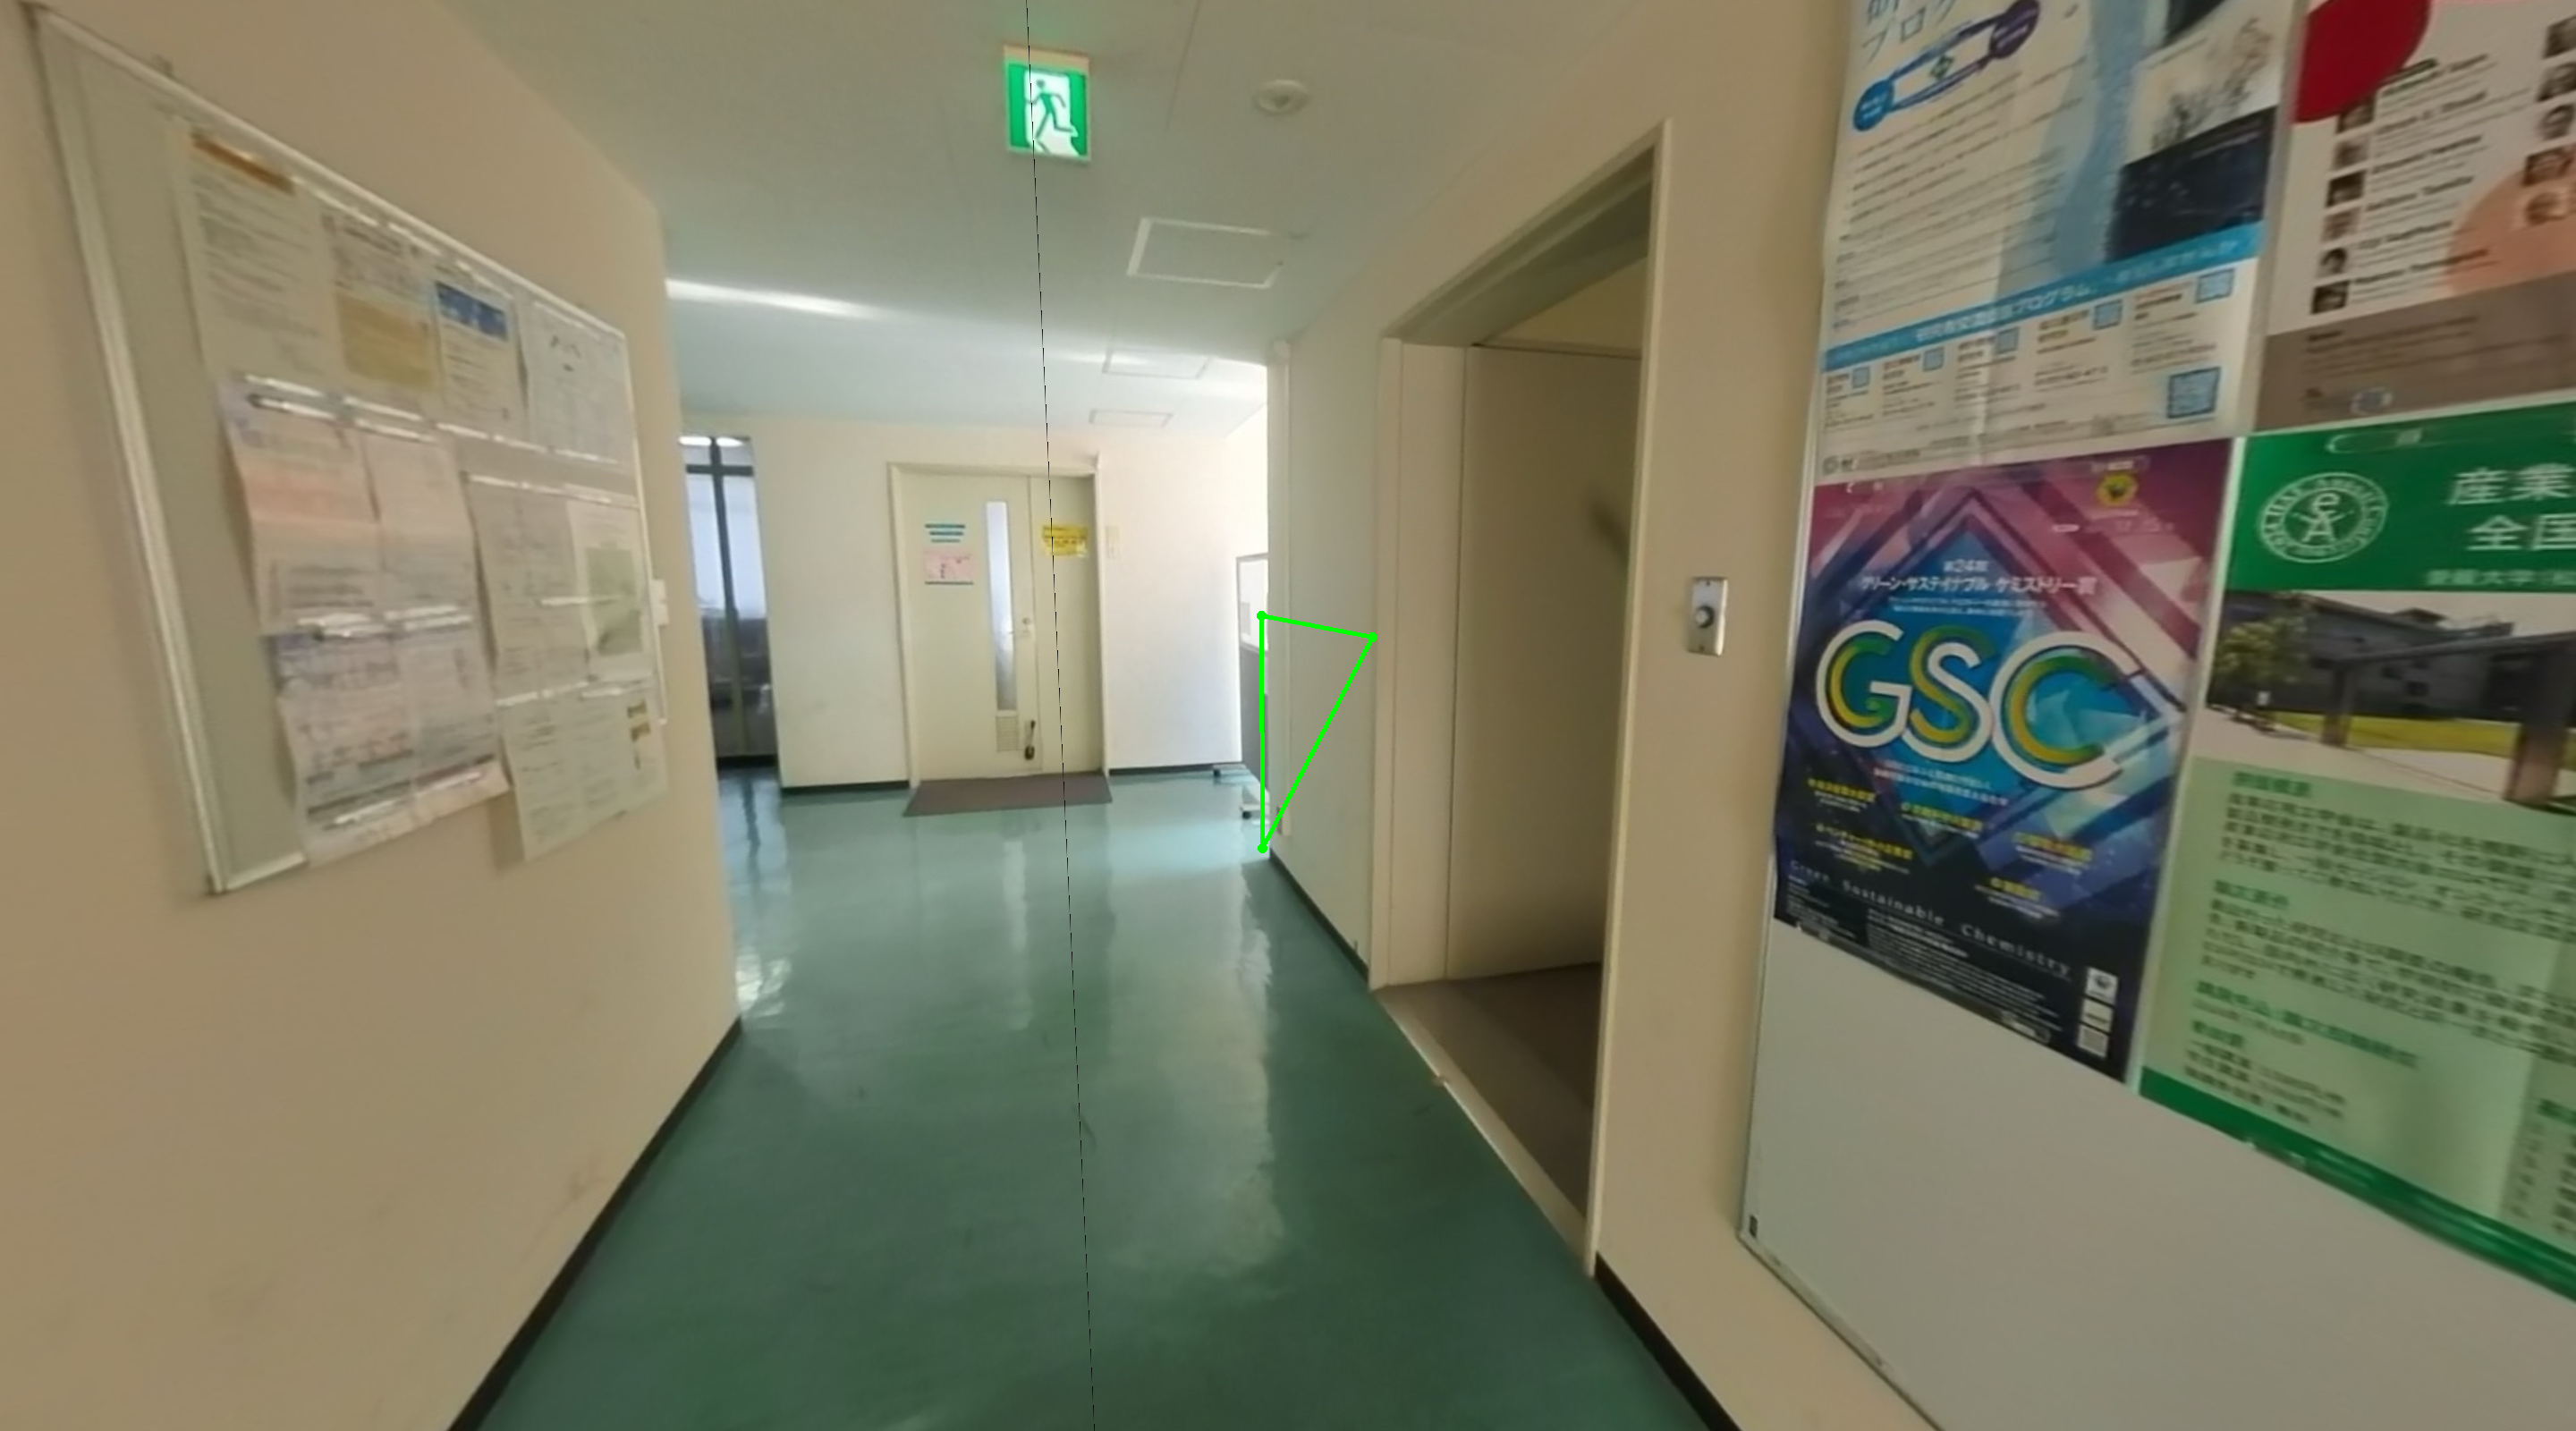
\includegraphics[width=0.3\textwidth]{figures/texture_1_15.png}&
      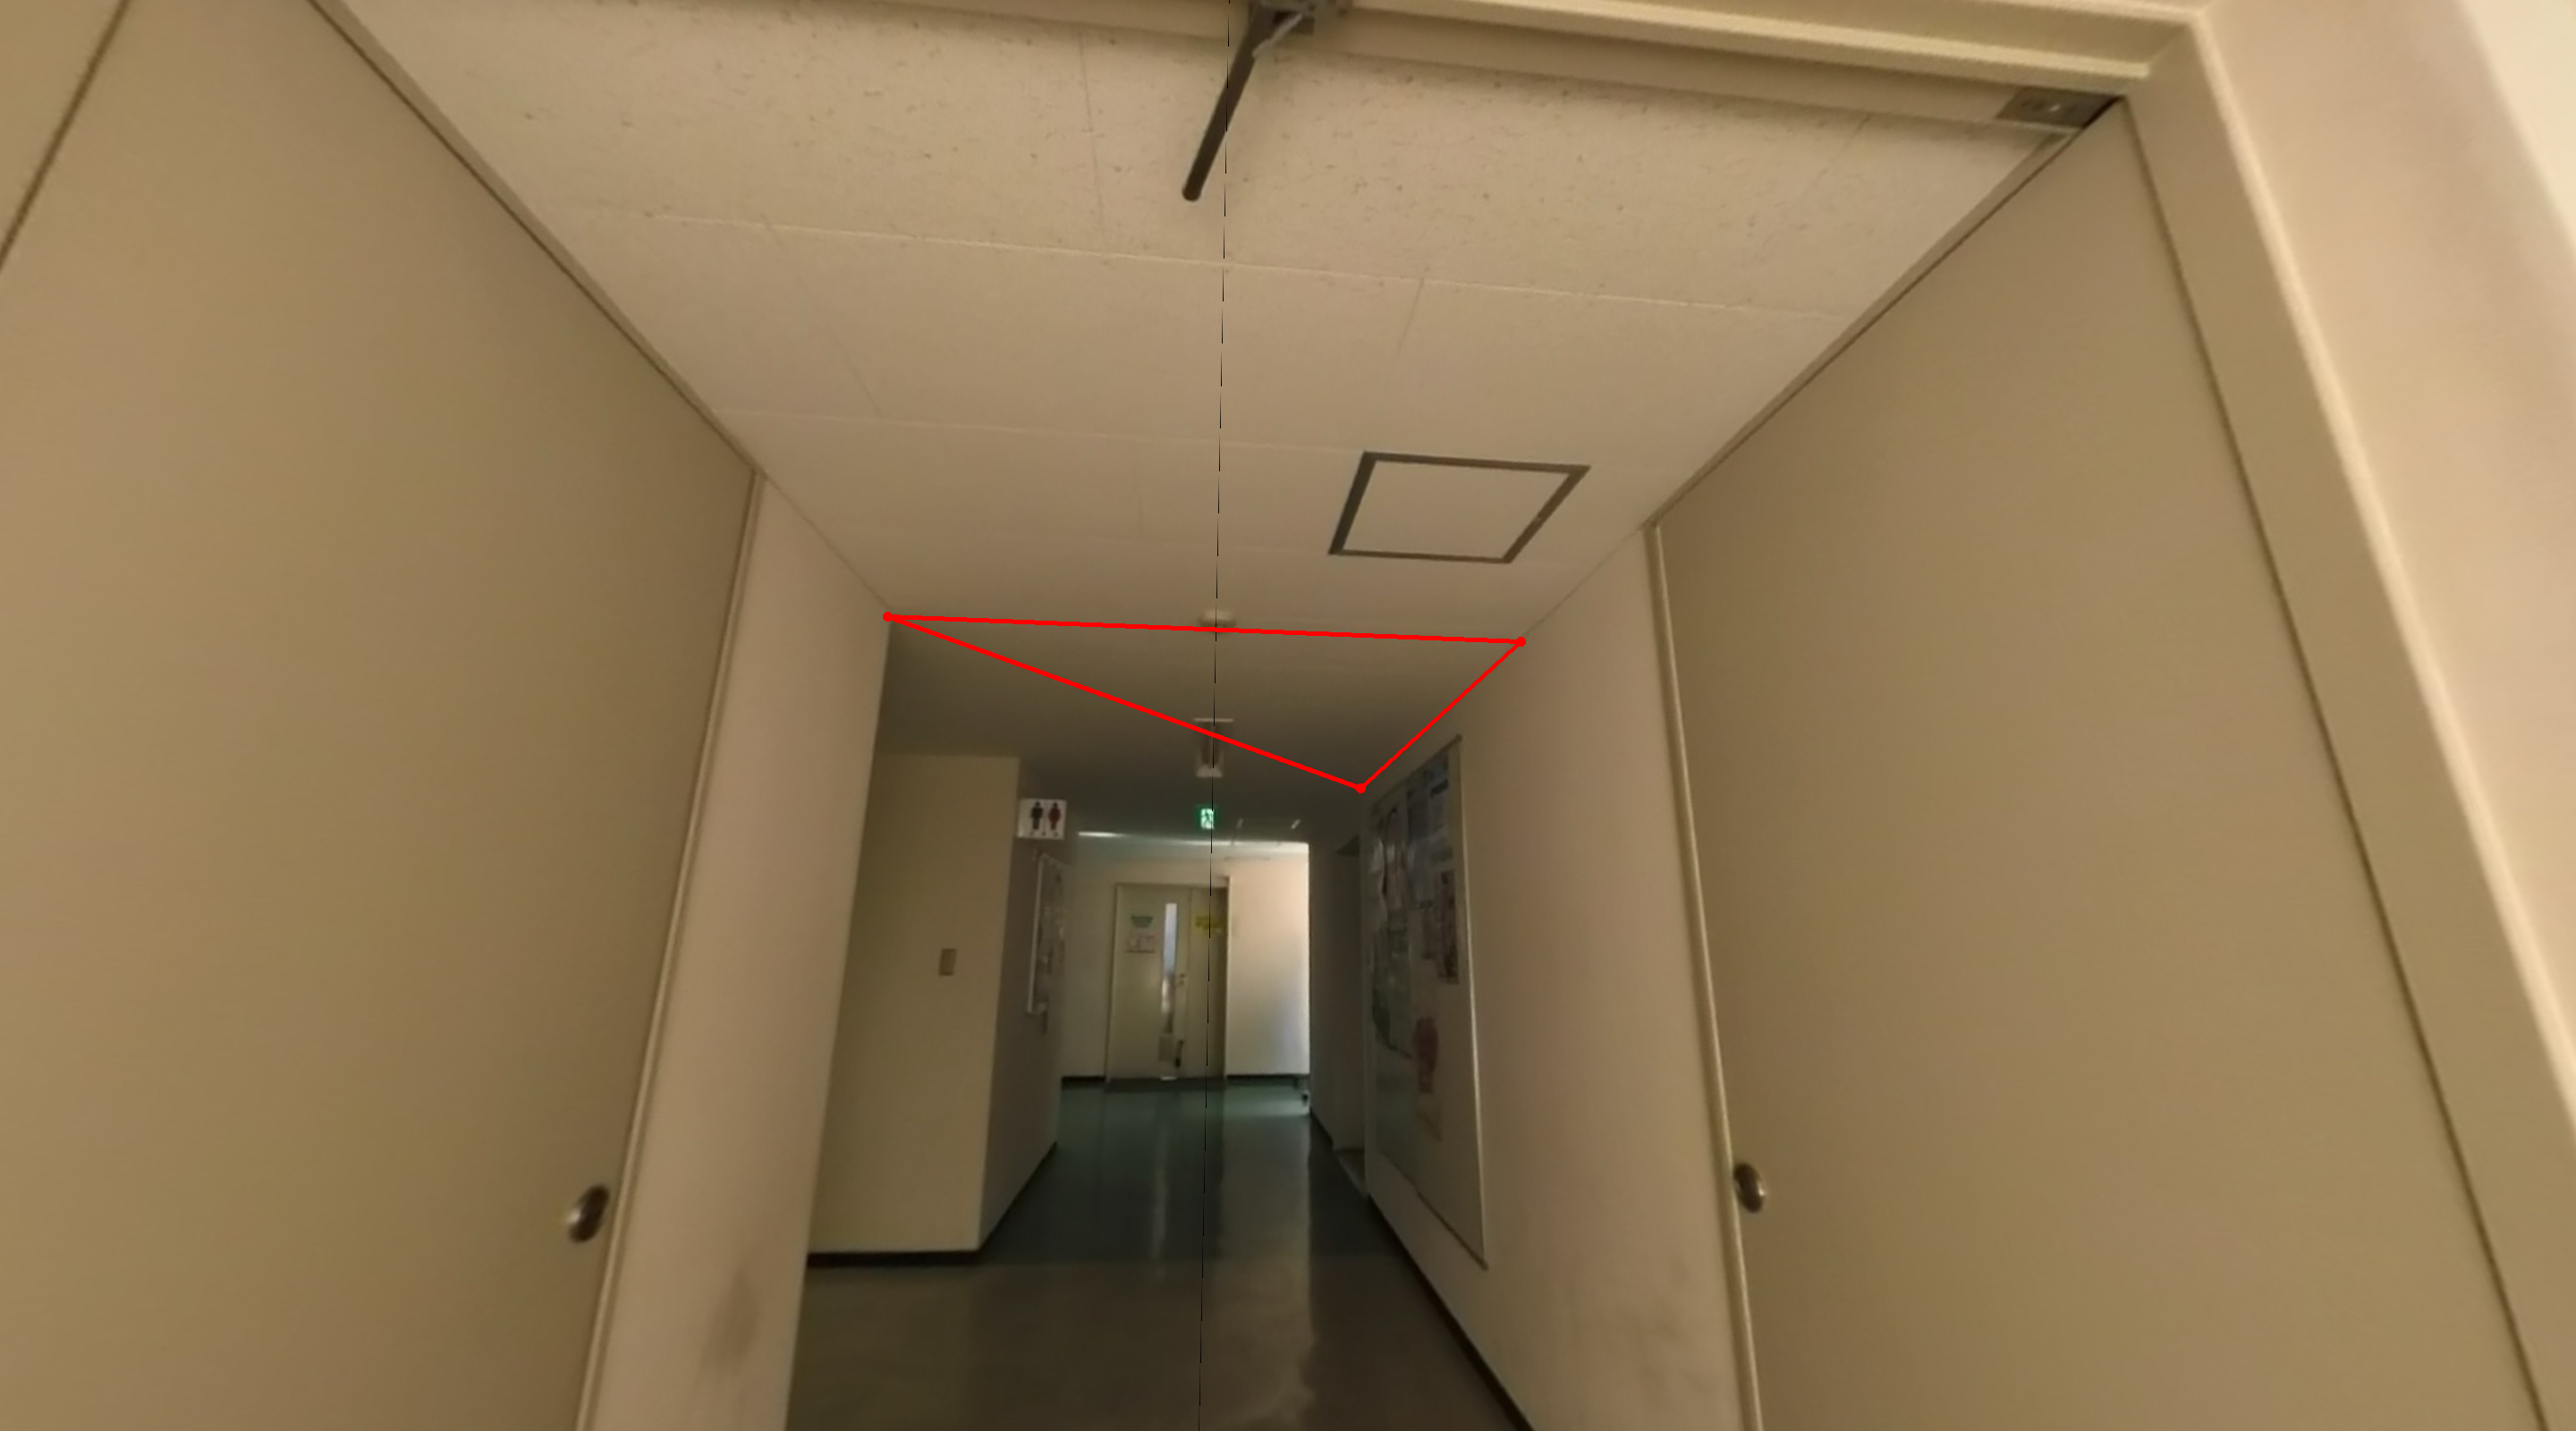
\includegraphics[width=0.3\textwidth]{figures/texture_2_5.png}\\
    \end{tabular}
  \end{center}
  \caption{テクスチャ画像}
  \label{one}
\end{figure}

\begin{figure}[H]
  \begin{center}
    \begin{tabular}{c}
      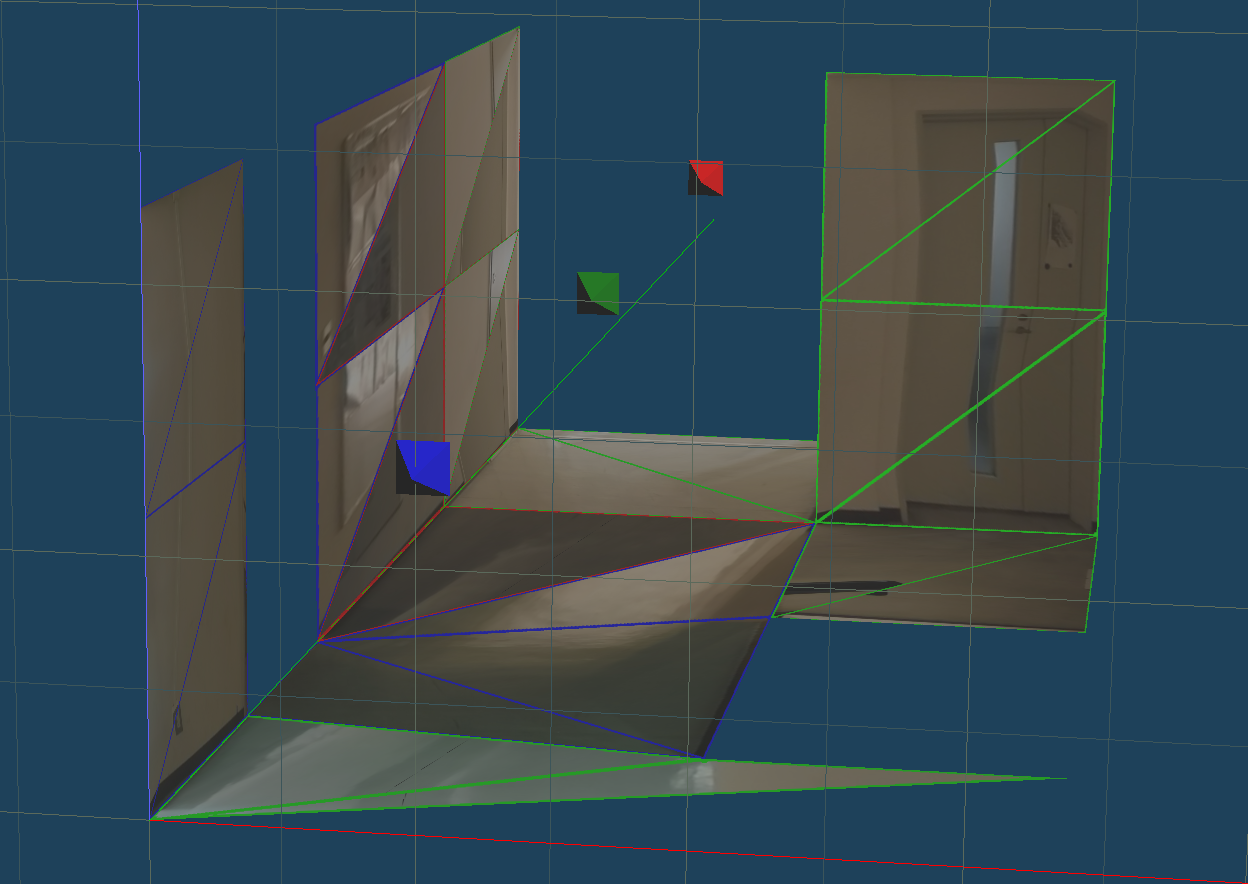
\includegraphics[width=0.7\textwidth]{figures/3dmodel012.png}
    \end{tabular}
  \end{center}
  \caption{3次元モデル(すべての全方位カメラ)}
  \label{two}
\end{figure}
これらの課題を解決するため、各テクスチャ間の輝度の差異を補正する必要があると考えた。
また、テクスチャ撮影時に用いた全方位カメラの配置が間隔的に広すぎたことがずれの原因と仮定し、カメラの配置を見直し、より密な間隔で再撮影を行う必要性があると判断した。
さらに、カメラパラメータを再計測し、取得するテクスチャの形状や大きさを適切に調整することで、3次元モデルの再現性が向上する可能性があると考えた。
今回の進捗報告では、これらの課題に対処すべく反映した変更点について説明するとともに、改良されたテクスチャを用いて生成した3次元モデルの結果を示す。
これにより、より再現度の高い3次元モデルの構築を目指す。

\section{テクスチャの明るさの差の改善}
全方位画像ごとに明るさに大きな差異が見られたため、それぞれの全方位画像を同じような明るさに調整するよう、改めて撮影を行った。
また、既存のテクスチャ間における明るさの差を低減させるため、以下のような具体的な手順を採用してテクスチャの輝度補正を実施した。
\begin{enumerate}
  \item 各テクスチャの三角形領域ごとの輝度平均をRGBの各成分について個別に計算
  \item 上の操作を全ての全方位画像について繰り返す
  \item 同一テクスチャの輝度平均を合計し、その値を全方位画像の枚数で除することで、目標となる輝度値(target brightness)を計算
  \item 個々のテクスチャにおける三角形領域内の輝度平均と、target brightnessの比率をスケール補正とする
  \item テクスチャとして採用する画像全体のRGB値にスケール補正を適用し、目標輝度に基づいて調整されたテクスチャ画像を生成
\end{enumerate}

\section{カメラ間隔の変更とカメラパラメータの再計測}
これらの結果により、全方位カメラ間のテクスチャずれの軽減を目的とした設計変更が効果的であることが示された。また、カメラ間隔の調整およびカメラパラメータの再計測が、3 次元モデル作成の精度向上に寄与する基盤となった。

異なる全方位カメラ間でテクスチャのずれが発生していた問題を改善するために、単一の全方位画像を用いた場合にはテクスチャのずれが発生しなかった点に着目した。
このことから、全方位カメラ間隔を縮小することで、テクスチャのずれを軽減できると考えた。
そのため、全方位カメラ間隔を近づけた状態で改めてテクスチャ作成用の全方位画像を撮影し、それに伴いカメラパラメータの再計測を実施した。
今回の撮影では、新しい全方位カメラ RICOH THETA X を採用した。
これは、以前使用していた Insta360 ONE X2 とは異なるカメラであるため、内部パラメータの再計測が必要であった。
内部パラメータ推定には、解像度$100\times100$の全方位画像を計 100 枚使用し、透視投影画像の画角を
$\theta=90°$、$\phi=90°$で、に設定して推定を行った。内部パラメータの推定結果は\hyperref[table1]{表\ref{table1}}に示す。
\begin{figure}[H]
  \begin{center}
    \begin{tabular}{lc}
    焦点距離fx & 0\\
    fy & 0\\
    光軸中心cx & 0\\
    cy & 0
    \end{tabular}
  \end{center}
  \caption{内部パラメータの推定結果}
  \label{table1}
\end{figure}

さらに、全方位カメラの位置と方向についても再設計を行い、その配置を\hyperref[three]{図\ref{three}}に示す。
この図において、赤い点はカメラパラメータ推定時に使用した2次元-3次元の対応点のxy平面上の位置を示している。
また、y軸で正の方向(0°)のカメラを基準カメラとして設定した。
中央に配置された全方位カメラでは、前方向で2方向(-30°、30°)、後ろ方向で3方向(150°、180°、-150°)を仮想カメラとして設定し、
計5つの視点を用いてカメラパラメータを推定している。
これにより、前回の設計に比べて仮想カメラの数を増加させたことで、カメラパラメータの推定精度向上が期待できる。
その他のカメラについては、後ろ方向(180°)のみ仮想カメラを用いている。
\begin{figure}[H]
  \begin{center}
    \begin{tabular}{c}
      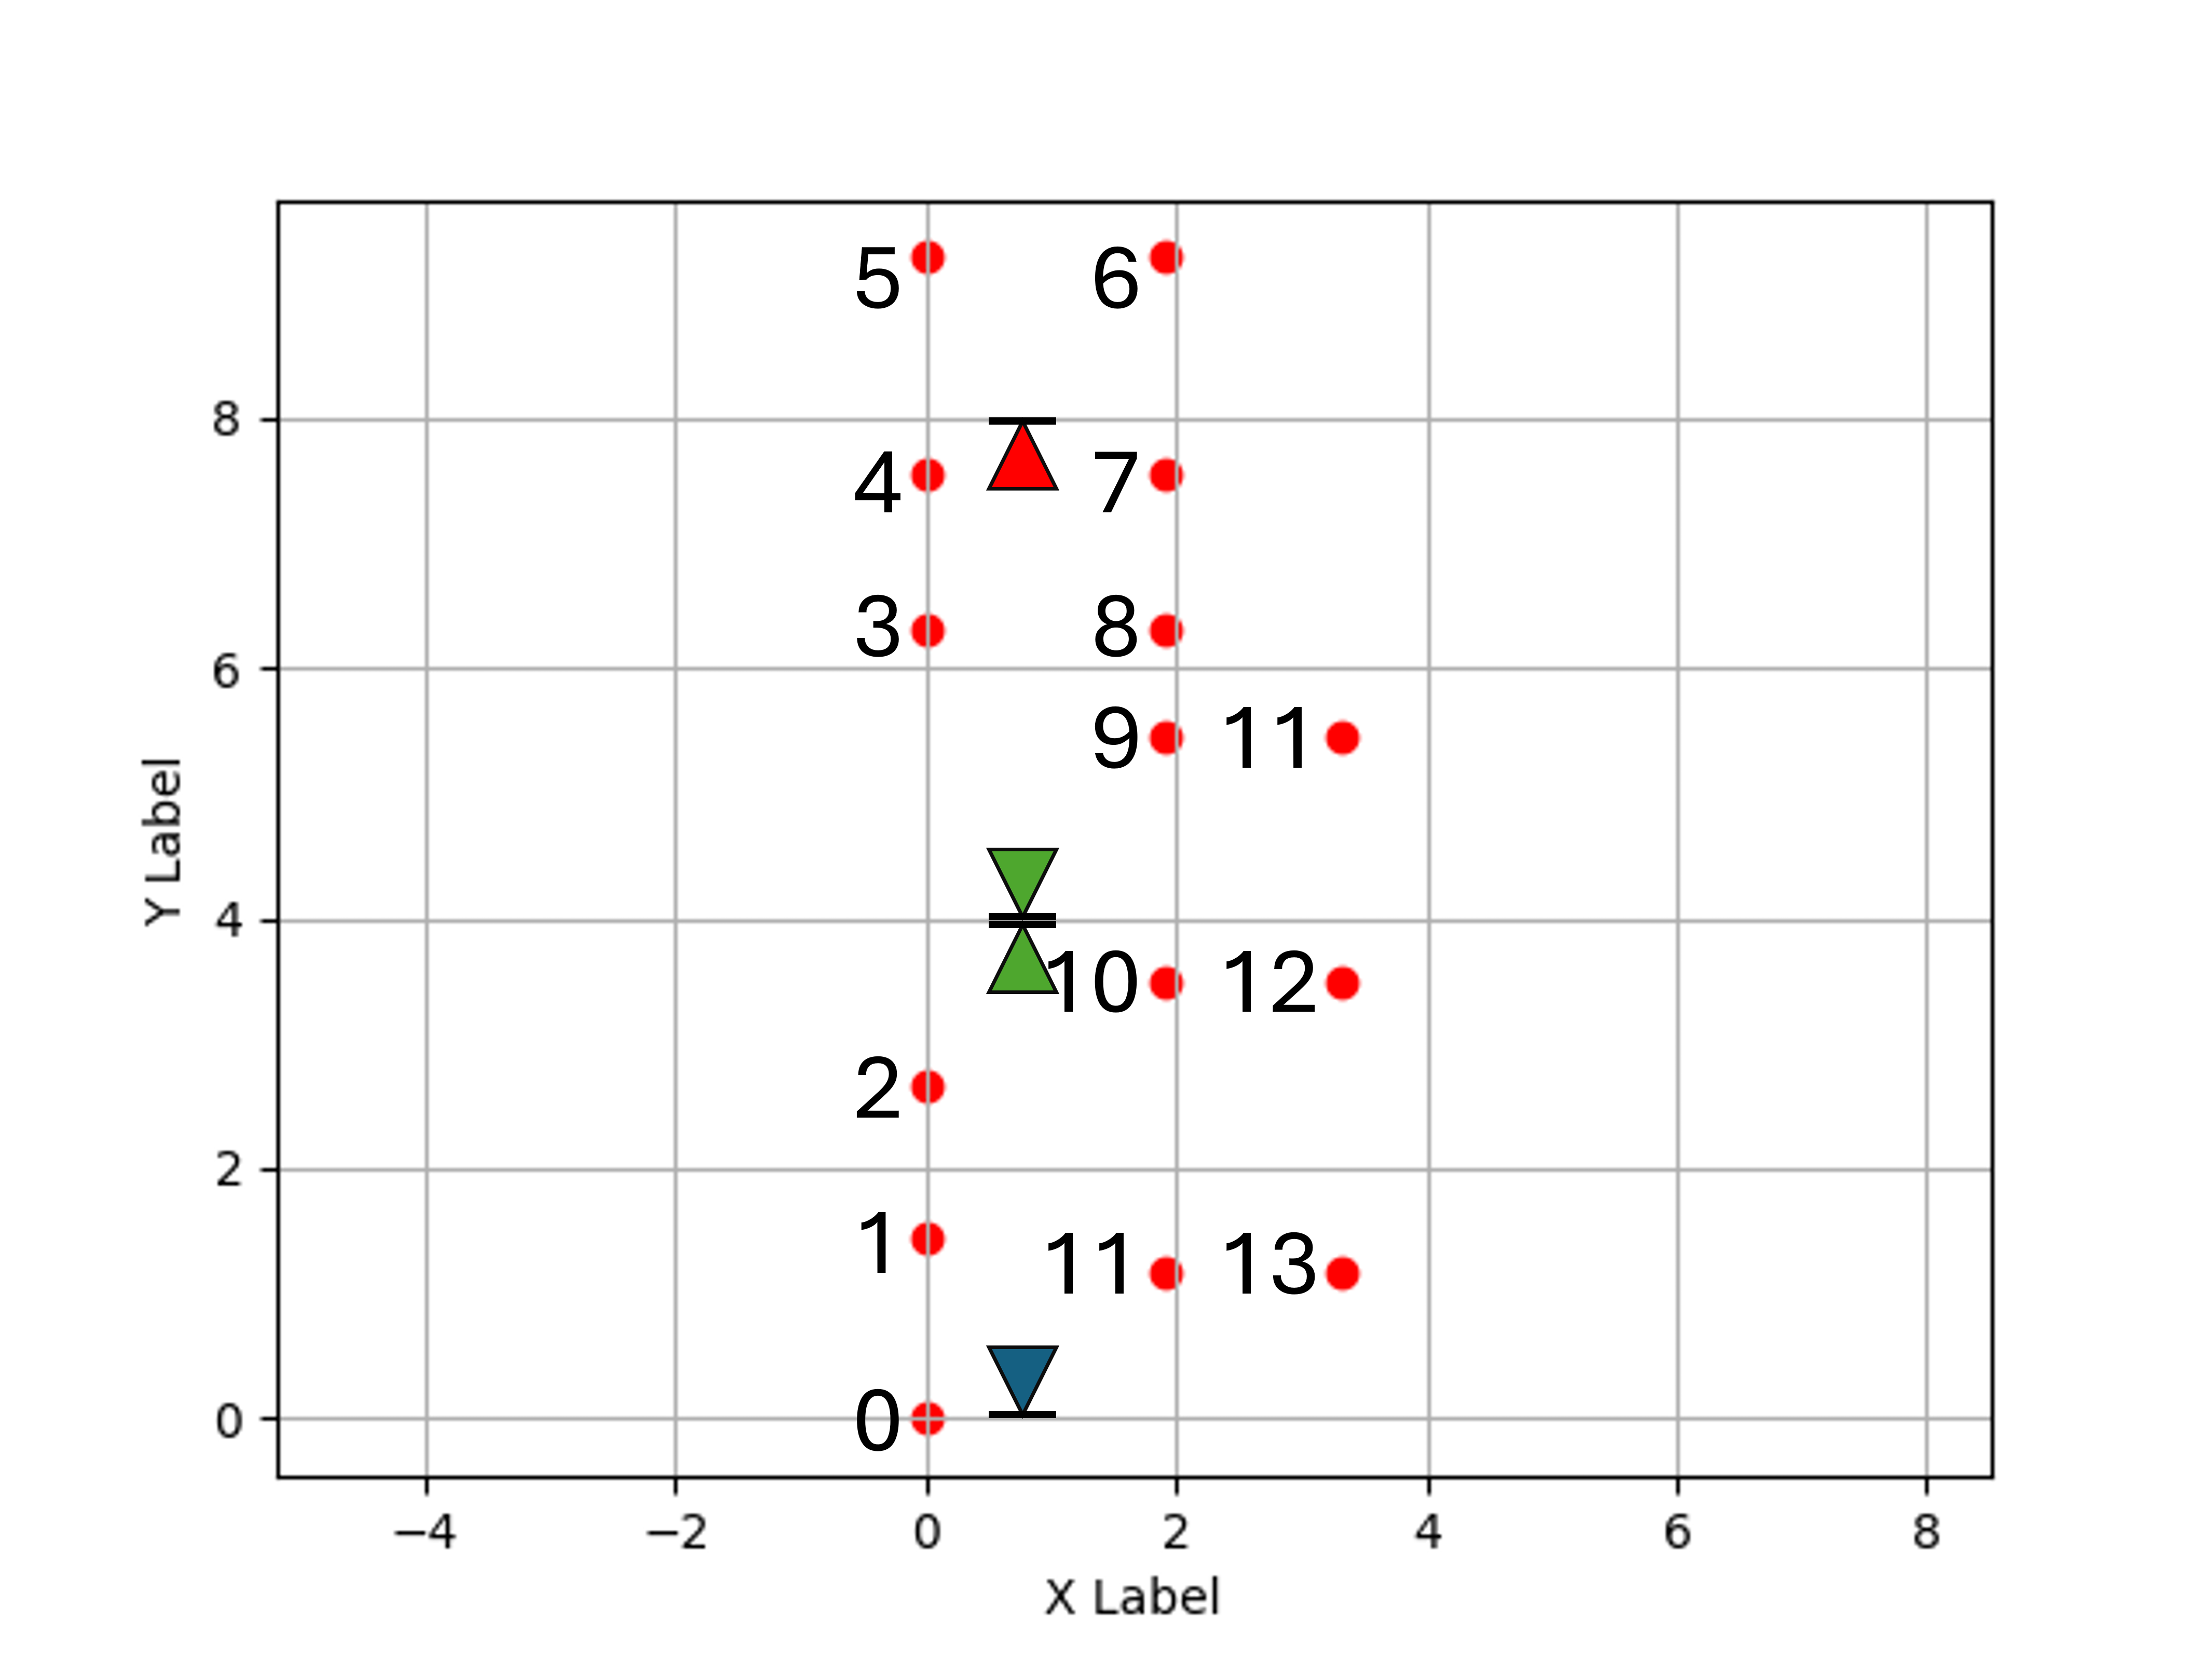
\includegraphics[width=0.5\textwidth]{figures/plot_campos.png}
    \end{tabular}
  \end{center}
  \caption{全方位カメラの位置、方向}
  \label{three}
\end{figure}

また、それぞれのカメラの外部パラメータ(並進ベクトル)の推定結果を\hyperref[table2]{表\ref{table2}}に示す。
\begin{figure}[H]
  \begin{center}
    \begin{tabular}{lccc}
    & 全方位カメラ0 & 全方位カメラ1 & 全方位カメラ2 \\
    誤差x(cm) & 99.9 & 100.0 & -0.1 \\
    誤差y(cm) & -6.2 & 0.0 & 6.2 \\
    誤差z(cm) & 134.3 & 136.0 & -1.6
    \end{tabular}
  \end{center}
  \caption{外部パラメータ(並進ベクトル)の推定結果}
  \label{table2}
\end{figure}
ここで、誤差は推定値と実測値の差であり、実測値には現実世界での計測誤差が含まれる点に留意する必要がある。
ただ、誤差についてはすべて1cm以下に収まっていて、かなり精度よくカメラパラメータを推定することができている。

\section{テクスチャの形状、大きさの変更}
ここまでの変更点を反映して作成された3次元モデルを\hyperref[four]{図\ref{four}}に示す。
この図から、明るさの差や底面のテクスチャのずれについては、一定の改善が見られる。
一方で、カメラ間隔を近づけた結果として、中心部分のテクスチャが取得できなくなる問題が新たに発生した。
この原因として、カメラと対象物(テクスチャ)の距離が近すぎるため、
透視投影画像内にすべてのテクスチャ三角形領域を描画するには視野角が過剰に大きくなることが挙げられる。

この問題を解決するため、テクスチャをより細かく分割する方法を採用した。
このアプローチによって、すべての面に対して必要なテクスチャを取得できると考えた。
ただし、テクスチャを細かく分割すると、各面のまとまりが小さくなり、視覚的な一体感が損なわれる可能性があるというデメリットも存在する。

\begin{figure}[H]
  \begin{center}
    \begin{tabular}{c}
      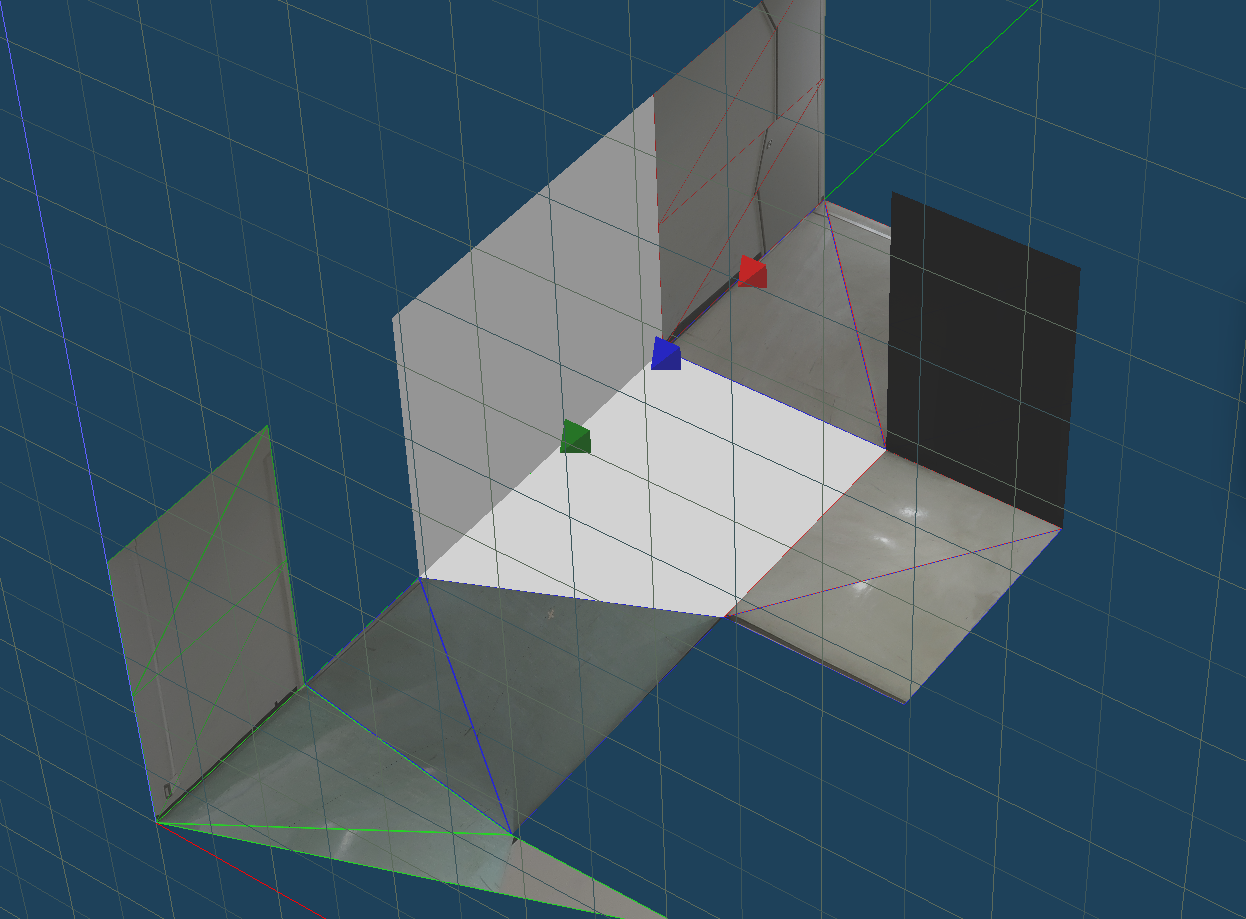
\includegraphics[width=0.7\textwidth]{figures/1.png}
    \end{tabular}
  \end{center}
  \caption{3次元モデル(すべての全方位カメラ)}
  \label{four}
\end{figure}

本研究では、2次元フロアマップを基にシーンの3次元モデルを構築することを目的としており、
その際に側面のテクスチャとしては店舗の正面や壁面が主な対象となると想定している。
店舗の正面や壁面は、一般的に直線的で角度がほとんどない面で構成されており、
これらの面を3次元モデル上で自然に再現するためには、テクスチャの形状についても直線的であることが望ましい。
そのため、側面のテクスチャの形状として四角形を採用することが最適であると判断した。
さらに、側面の四角形テクスチャについては、3次元モデル作成時の歪みを軽減するため、
ホモグラフィー変換を適用し長方形となるよう補正を行った。
これらのテクスチャ画像を\hyperref[five]{図\ref{five}}に示す。

\begin{figure}[H]
  \begin{center}
    \begin{tabular}{cc}
      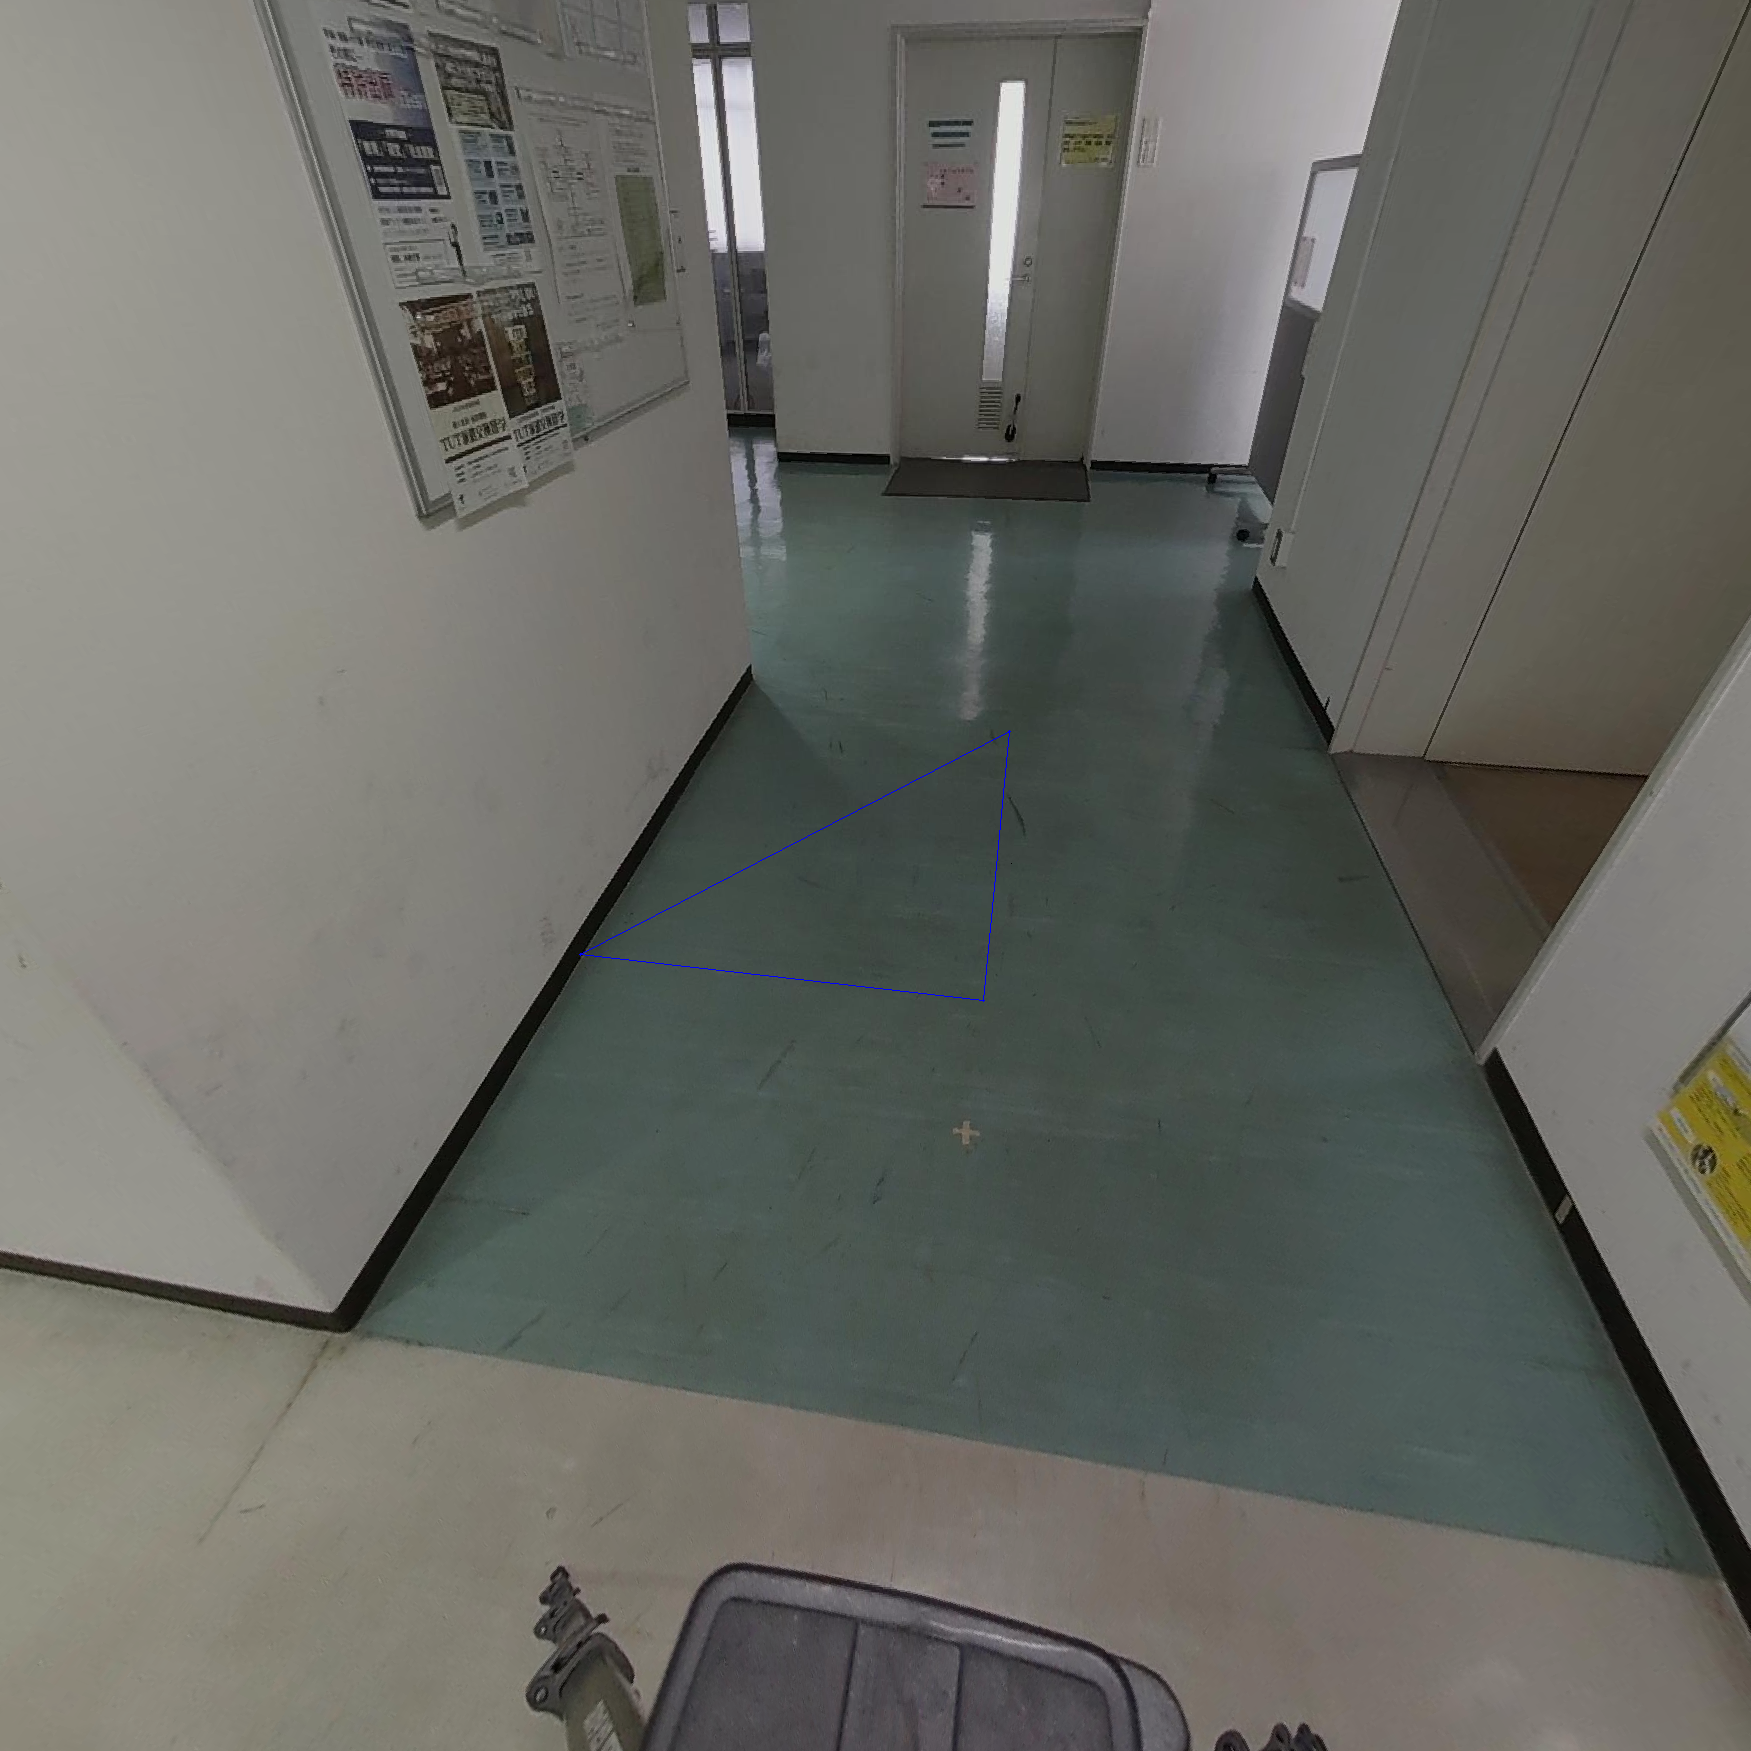
\includegraphics[width=0.4\textwidth]{figures/texture_0_6.png}&
      \includegraphics[width=0.4\textwidth]{figures/texture_0_46.png}\\
      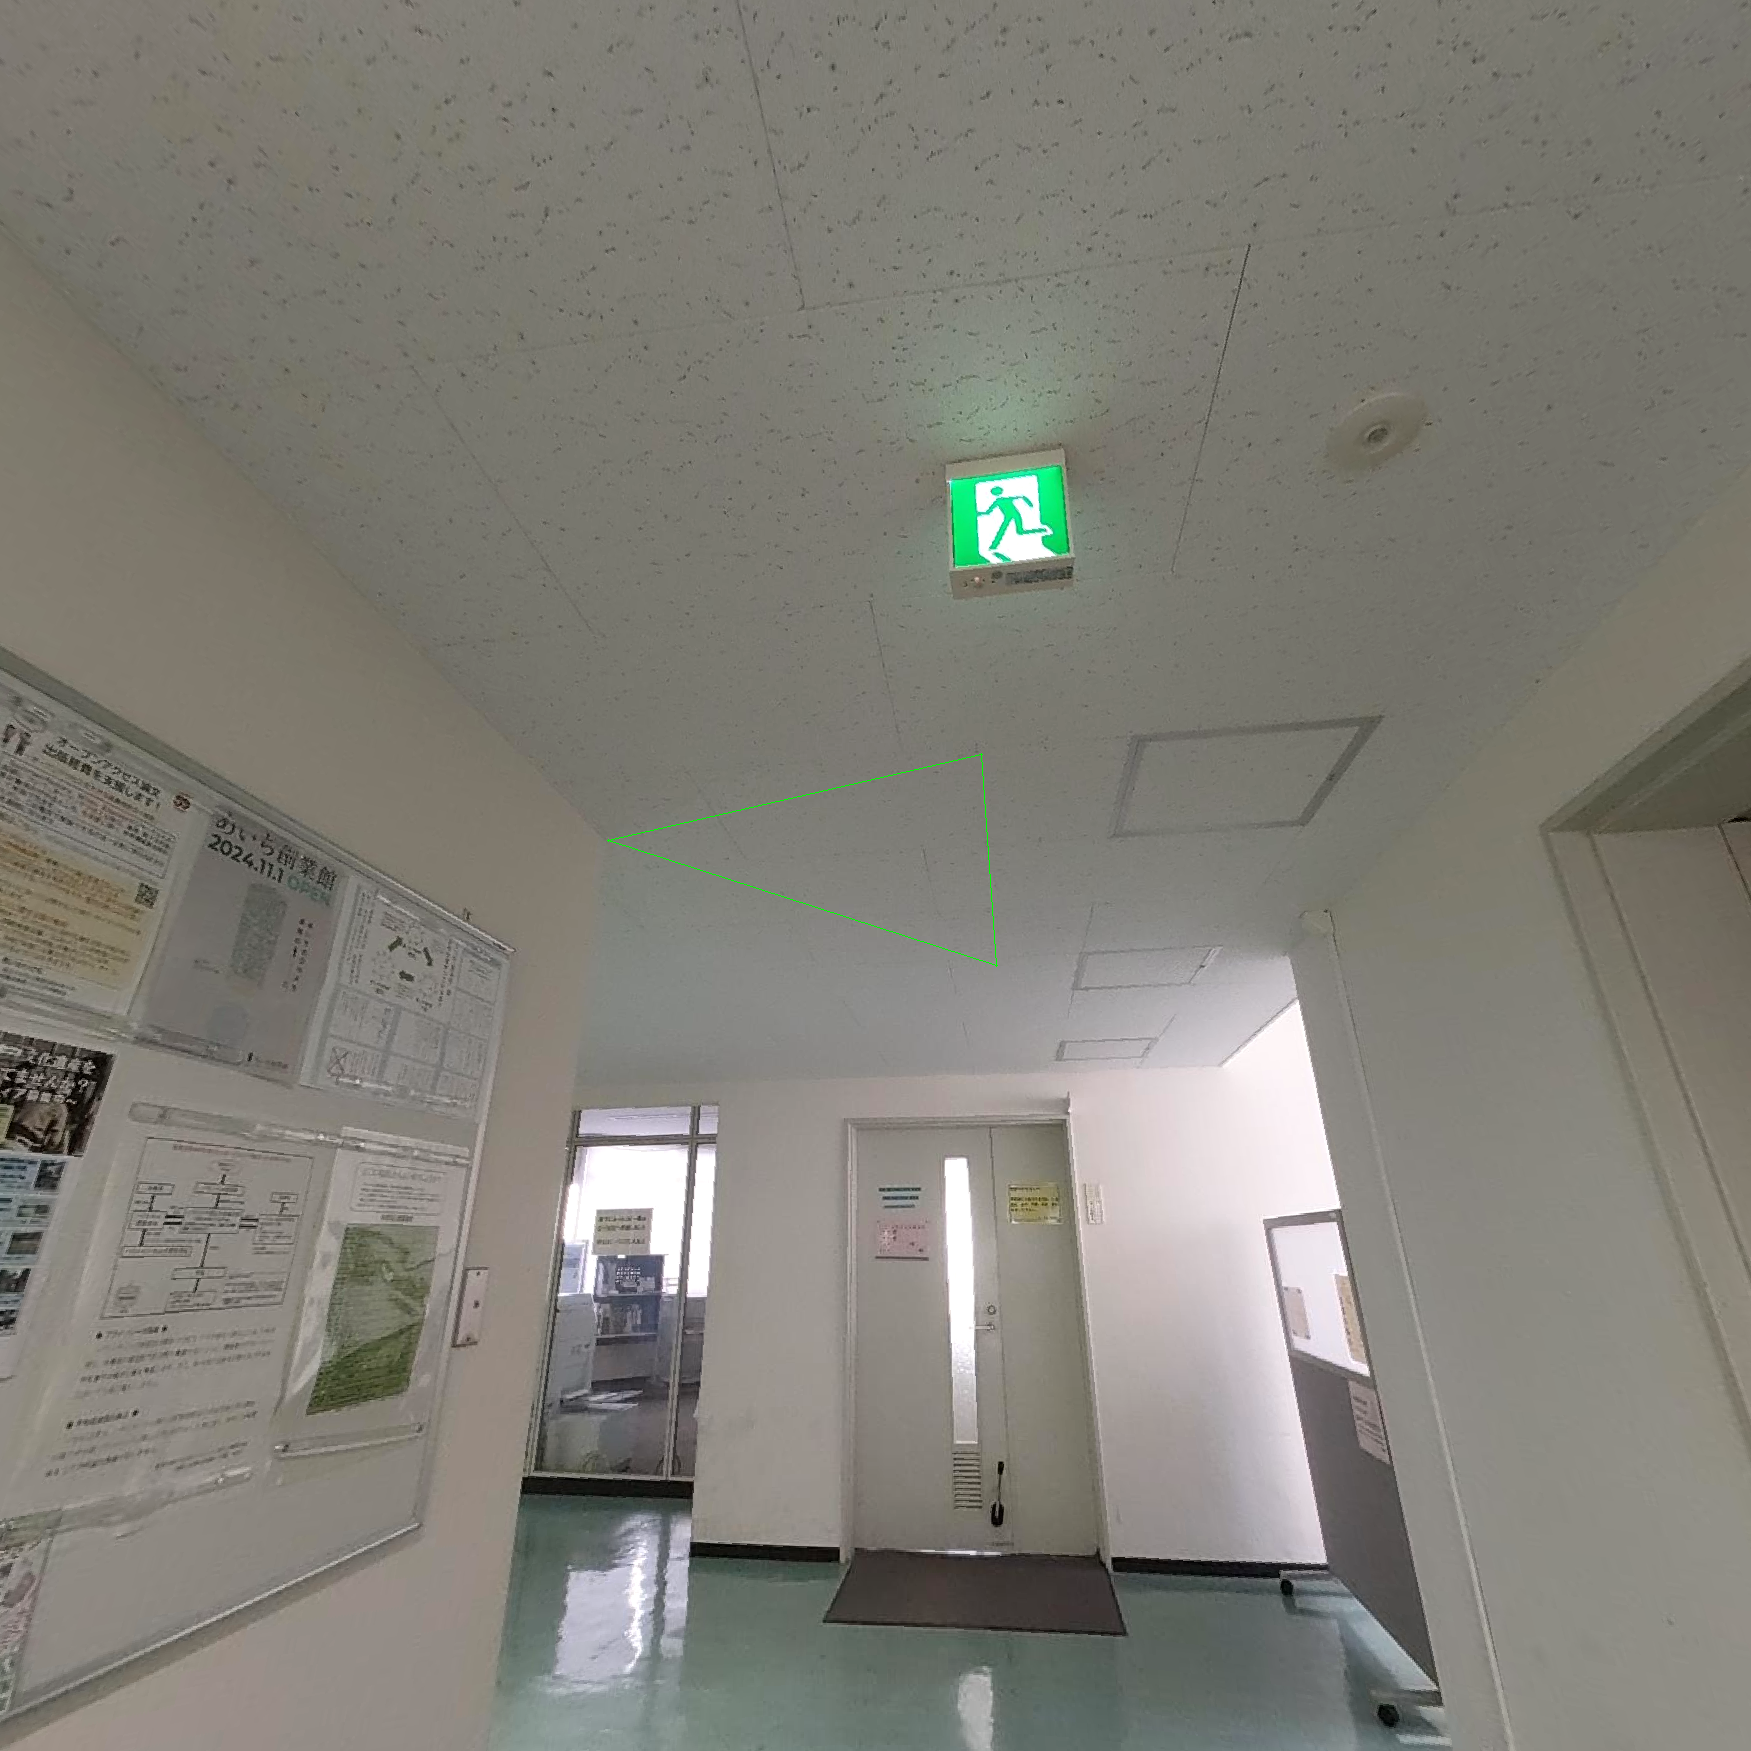
\includegraphics[width=0.4\textwidth]{figures/texture_1_24.png}&
      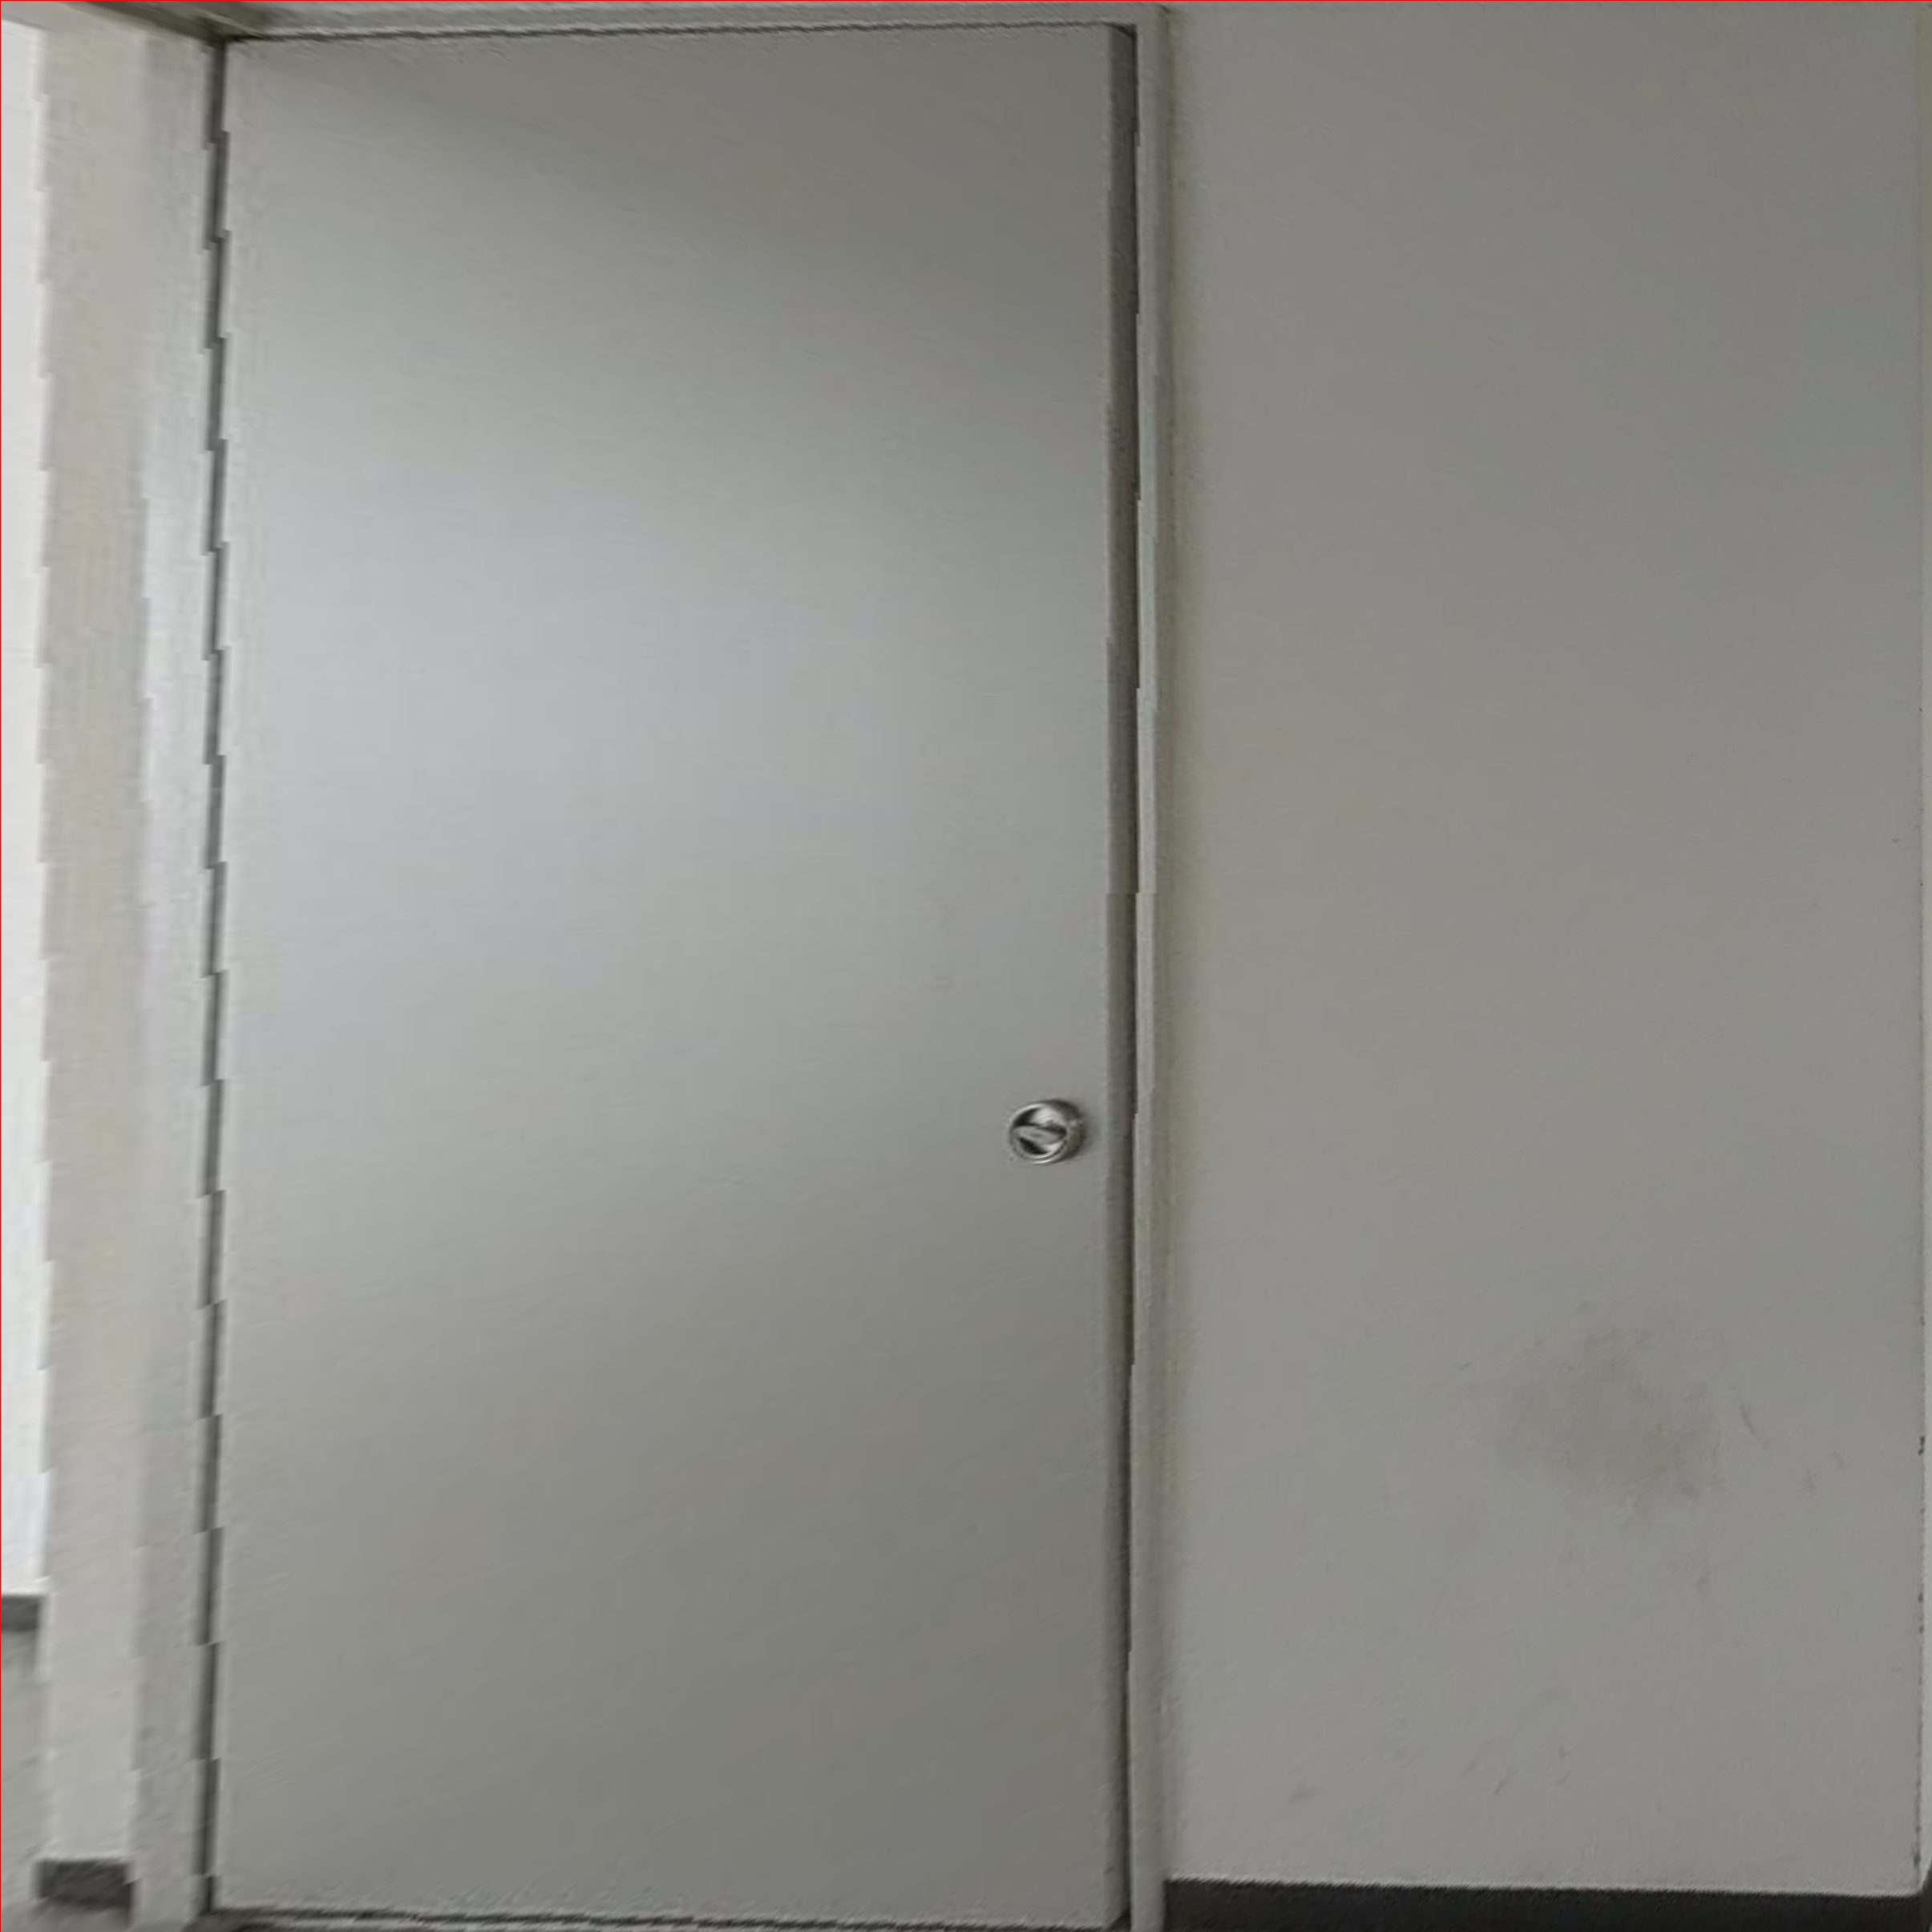
\includegraphics[width=0.4\textwidth]{figures/texture_2_54.png}\\
    \end{tabular}
  \end{center}
  \caption{テクスチャ画像}
  \label{five}
\end{figure}

これらのテクスチャを用いて生成した3次元モデルを\hyperref[six]{図\ref{six}}に示す。
このモデルでは、テクスチャの形状を改善したことにより、すべての面に対して適切なテクスチャを取得することが可能となった。
また、側面のテクスチャについても四角形テクスチャを採用することで、滑らかで視覚的に一貫性のある表現を実現した。

\begin{figure}[H]
  \begin{center}
    \begin{tabular}{c}
      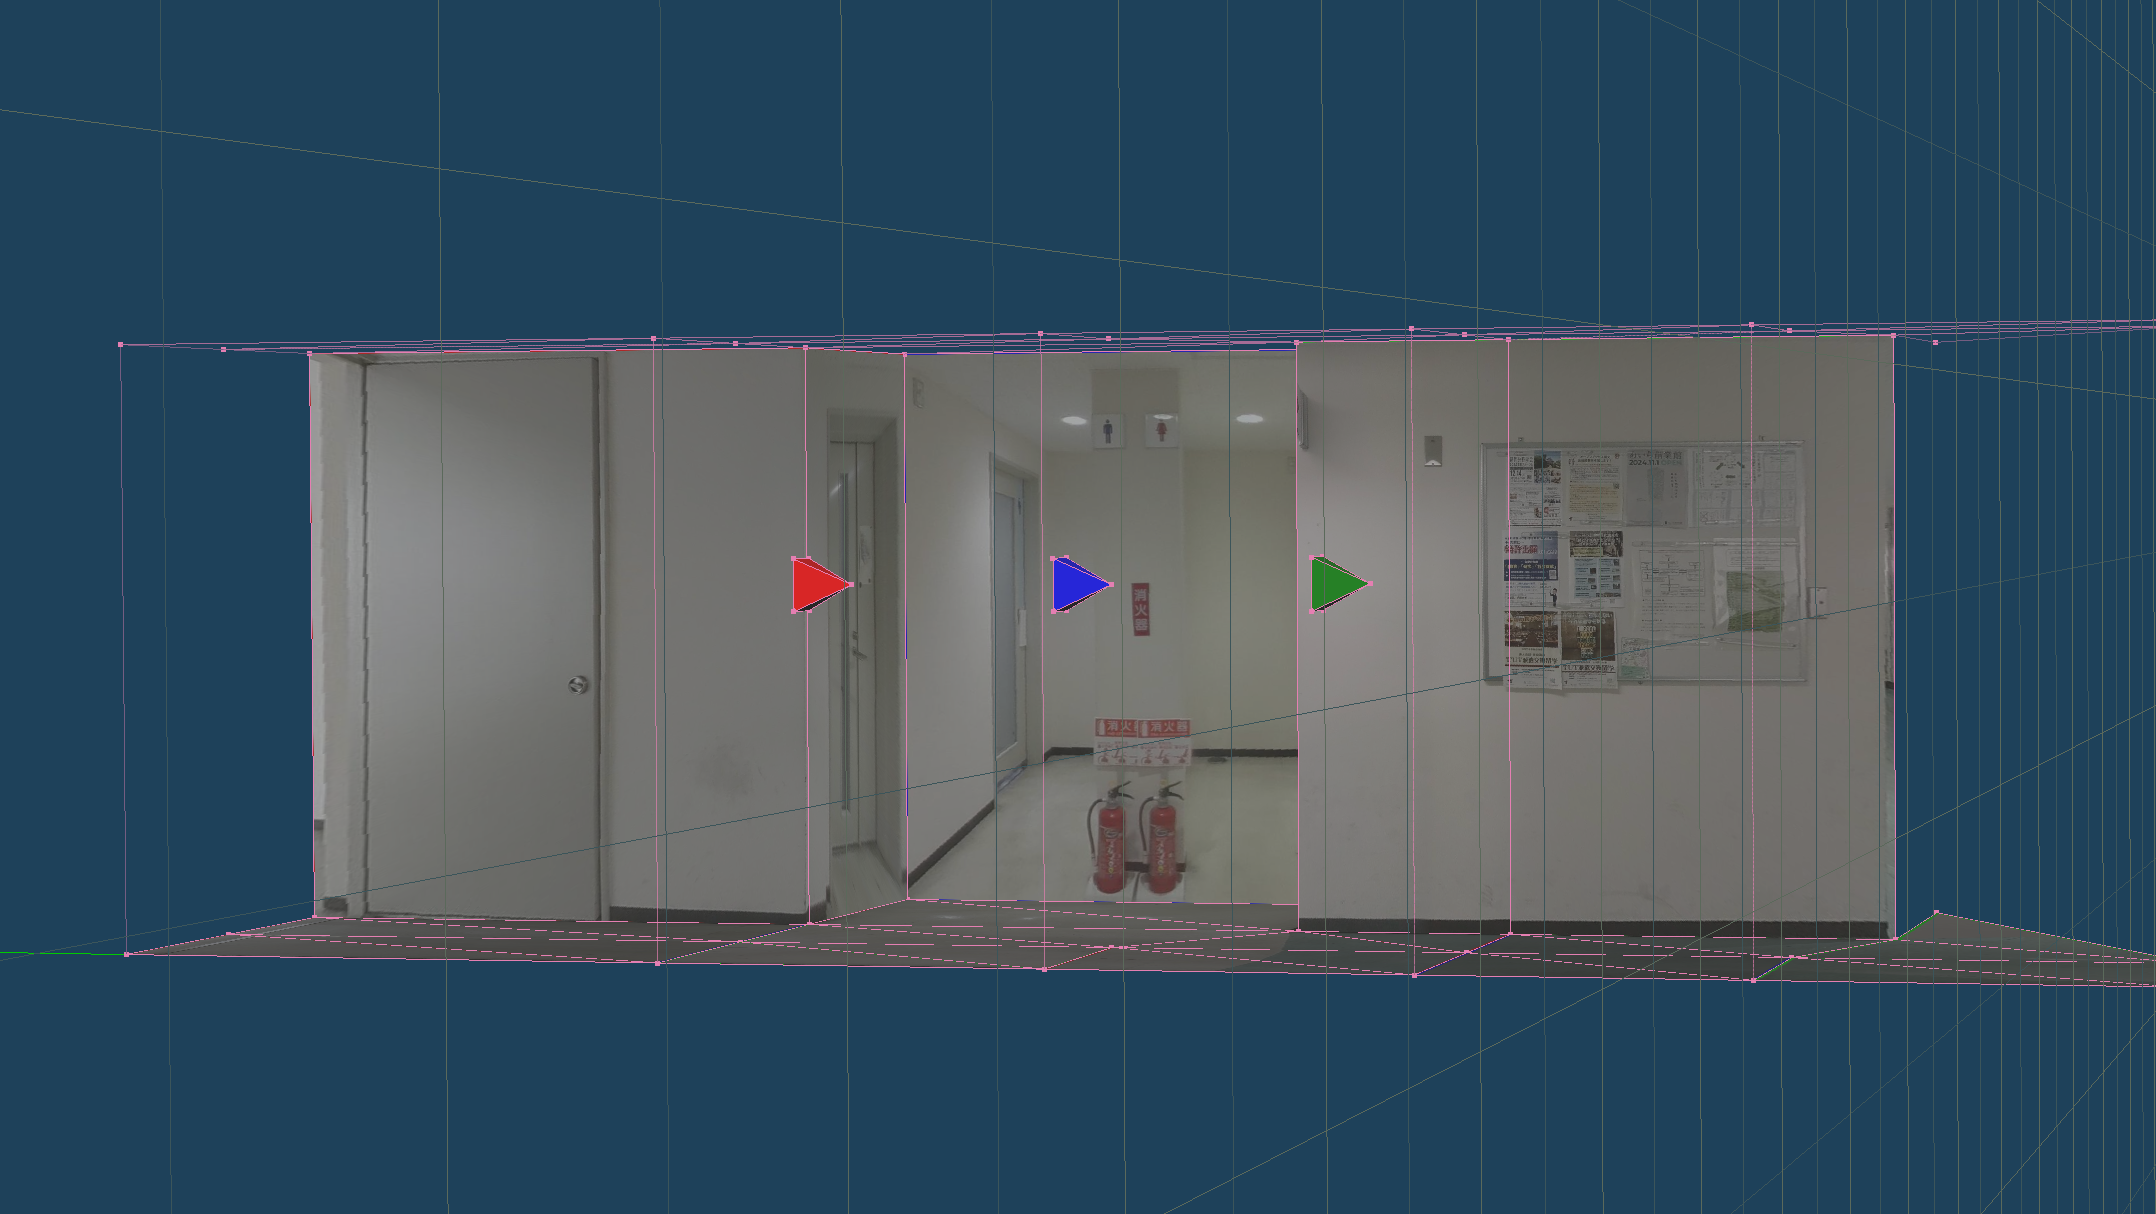
\includegraphics[width=0.7\textwidth]{figures/2.png}\\
      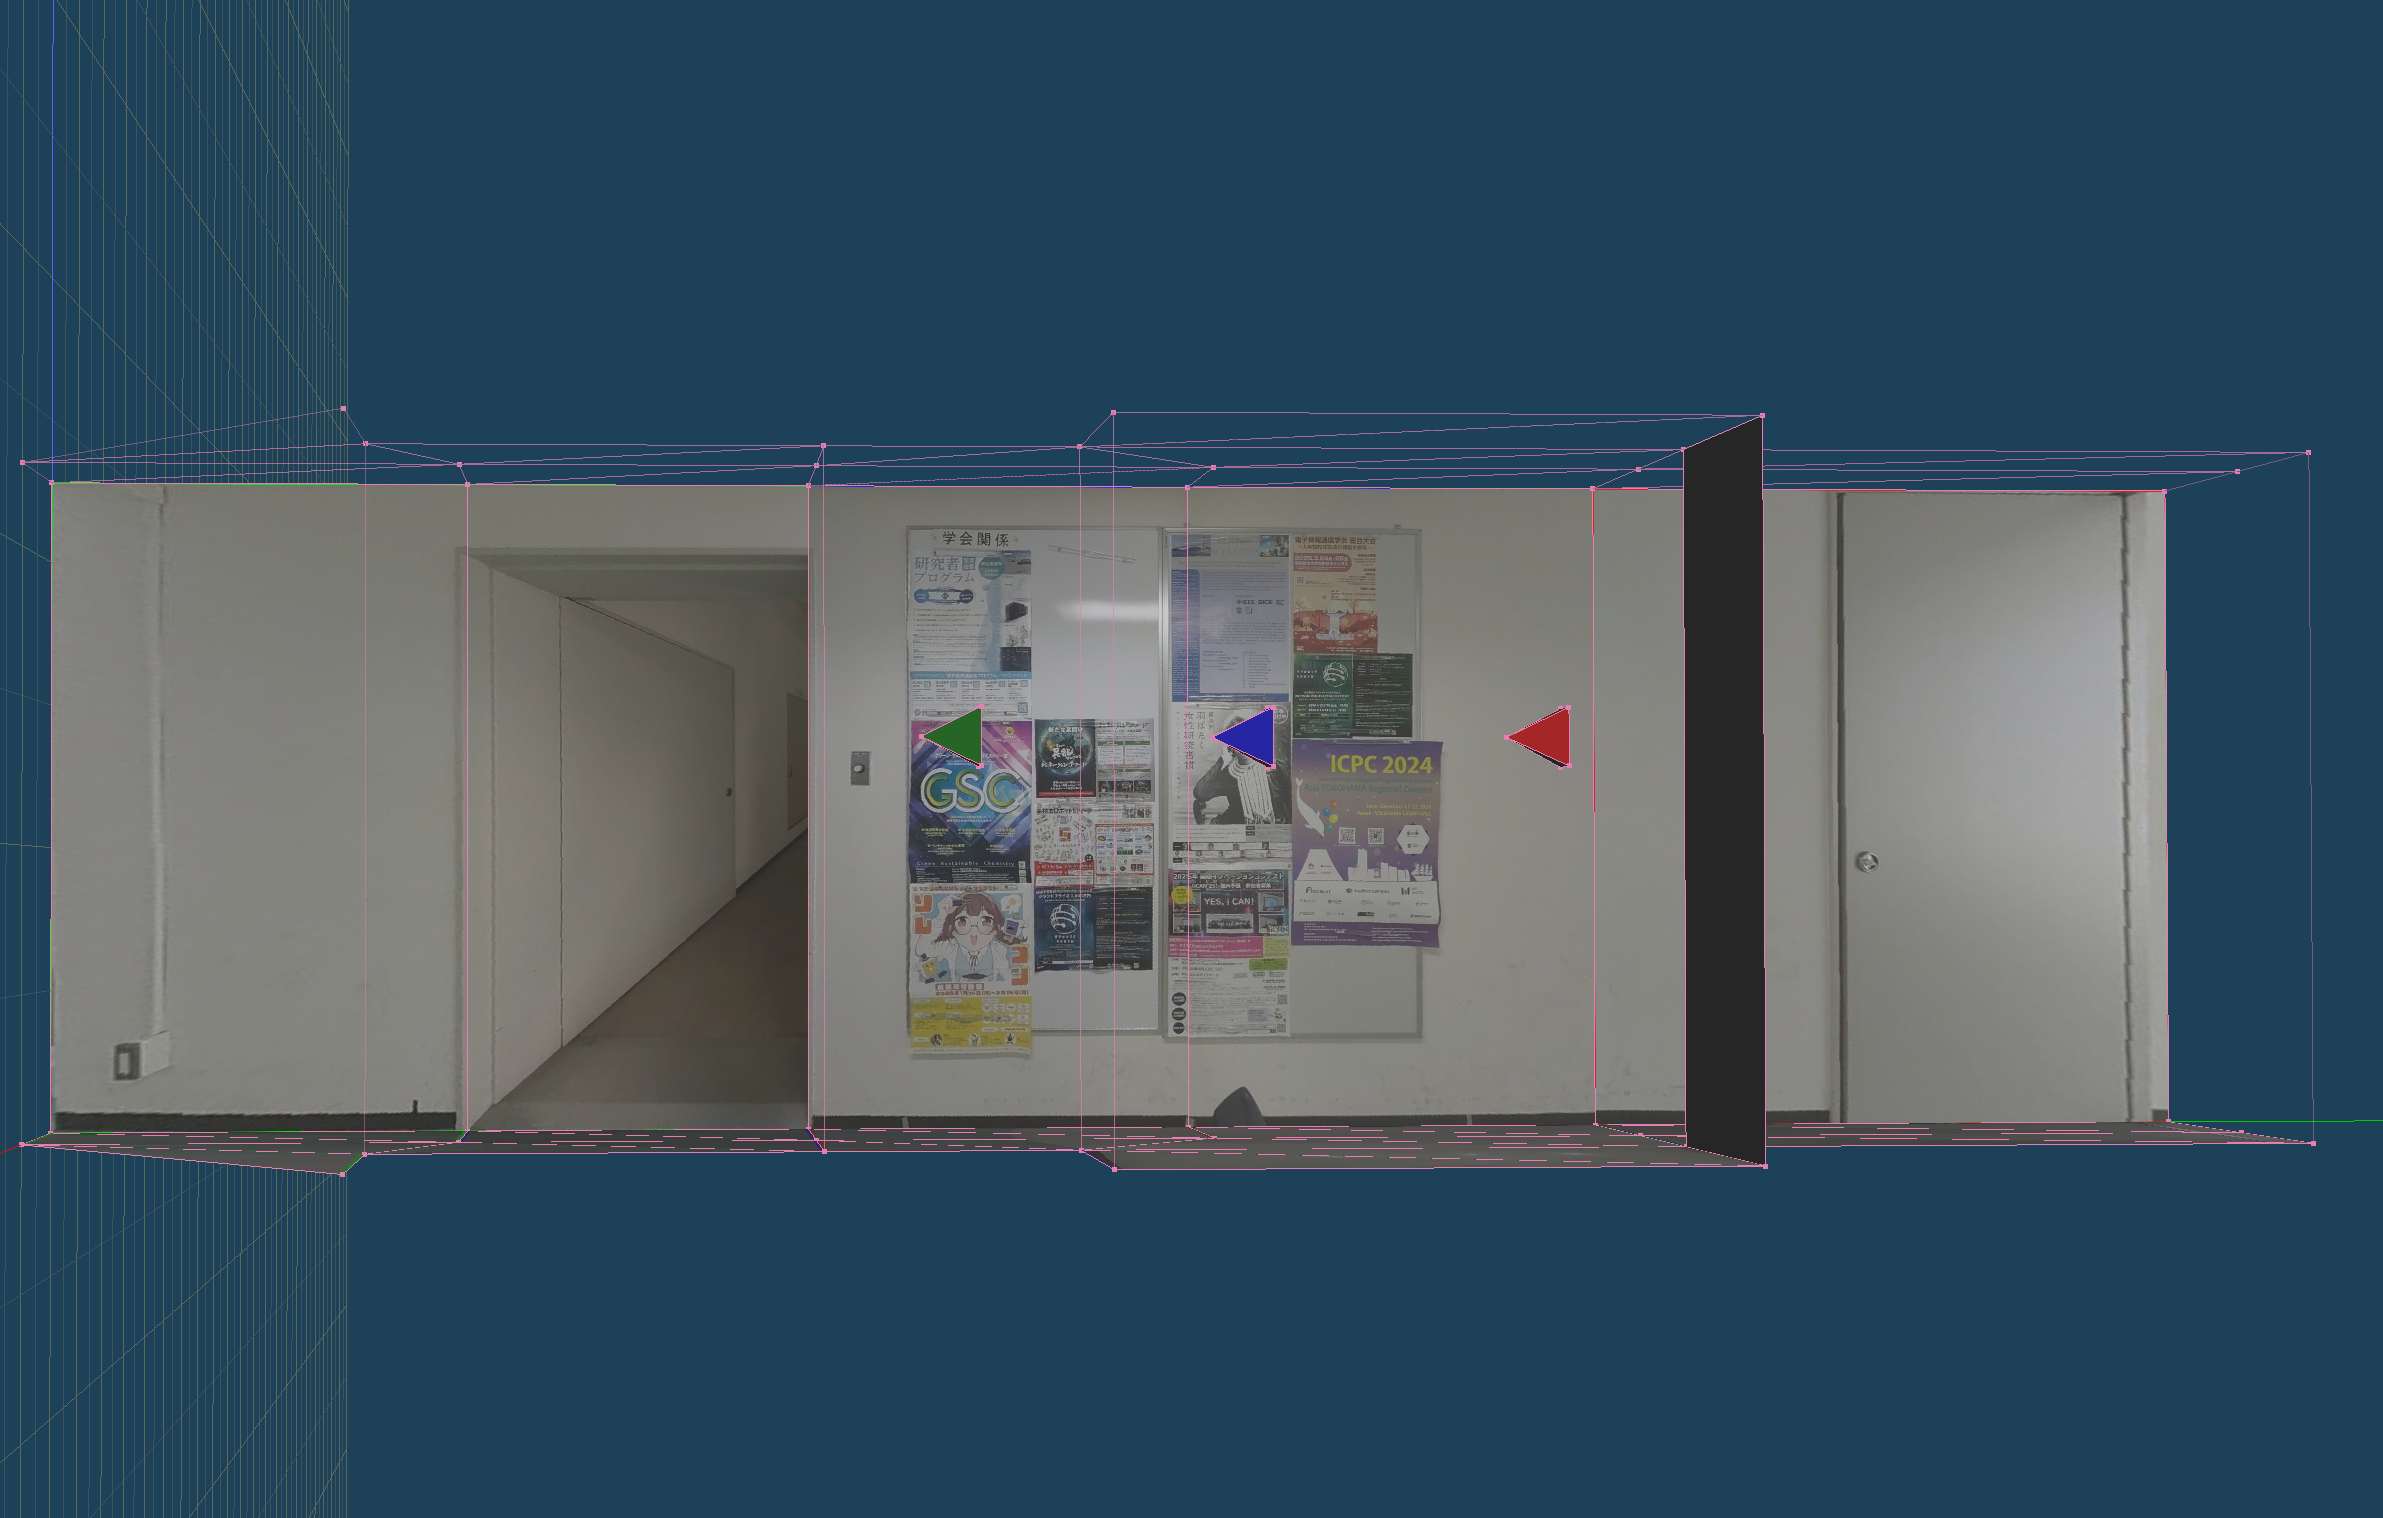
\includegraphics[width=0.7\textwidth]{figures/3.png}\\
      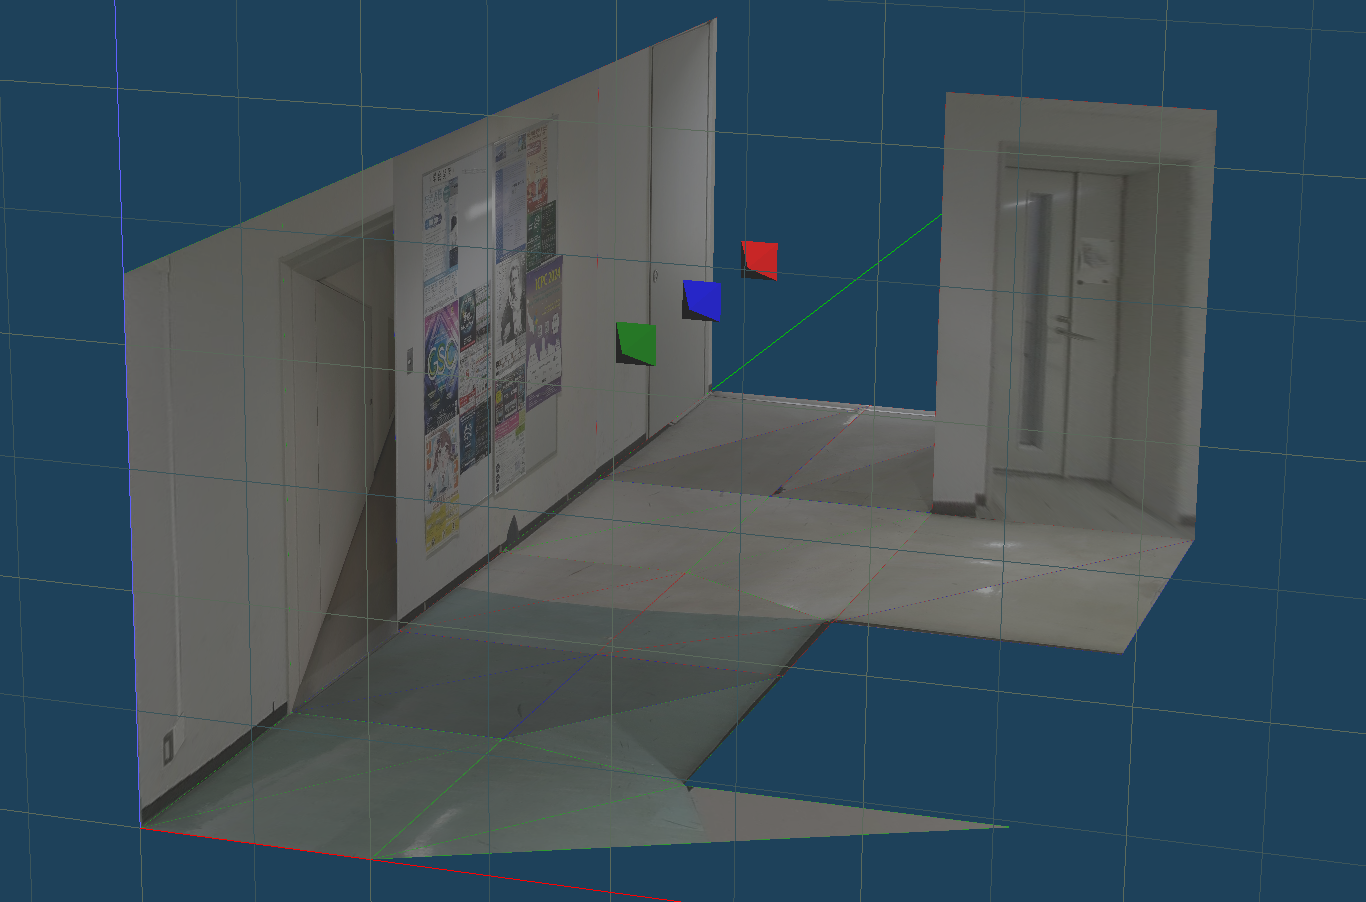
\includegraphics[width=0.8\textwidth]{figures/4.png}\\
    \end{tabular}
  \end{center}
  \caption{3次元モデル}
  \label{six}
\end{figure}

\section{今後の目標}
現在、3次元モデルの再現度については一定の成果を得ることができたため、
今後は作成した3次元モデルを活用した自己位置推定手法の検討を進める。
具体的には、テクスチャから得られる色情報を使用しない自己位置推定と、テクスチャの色情報を利用した自己位置推定を比較し、
色情報の有無が推定精度に与える影響を明らかにする予定である。
これにより、テクスチャ情報が自己位置推定においてどの程度有益であるかを定量的に評価できると考える。
さらに、実際の自己位置と推定位置との誤差を比較することで、自己位置推定の精度を検証する。
この結果を踏まえて、推定精度が実用的な範囲に収まっているかどうか、実際のアプリケーションにおいて
どのような精度が求められるかについても考察する予定である。
\end{document}
